\documentclass[aspectratio=169, xcolor=dvipsnames]{beamer}
\usepackage{changepage}
\usepackage{fontspec}
\usepackage{caption}
\usepackage{amsmath}
\usepackage{annotate-equations}

% \usepackage[style=apa]{biblatex}

% % Add bibliography file
% \addbibresource{bibliography.bib}


% Define fonts
\setsansfont{SourceSerif4}[
    Path=./static/,
    Extension = .ttf,
    UprightFont=*-Regular,
    BoldFont=*-Bold,
    ItalicFont=*-Italic,
    BoldItalicFont=*-BoldItalic,
    SlantedFont=*-ExtraLight,
    ]

% Define colours
\definecolor{lightBlue}{RGB}{129, 183, 242}
\definecolor{lightGrey}{RGB}{128, 128, 128}
\definecolor{lightRed}{RGB}{255, 143, 143}
\definecolor{lightGreen}{RGB}{46, 184, 59}
\definecolor{lightPurple}{RGB}{160, 98, 239}
\definecolor{blue}{RGB}{0, 56, 101}
\definecolor{grey}{RGB}{180, 180, 180}
\definecolor{red}{RGB}{255, 0, 0}
\definecolor{white}{RGB}{255, 255, 255}
\definecolor{black70}{gray}{0.3}

% Define beamer theme
\setbeamercolor{title page}{bg=blue}
\setbeamercolor{title}{fg=red}
\setbeamercolor{frametitle}{fg=blue}
\setbeamercolor{subtitle}{fg=grey}
\setbeamercolor{author}{fg=grey}
\setbeamercolor{date}{fg=grey}
\setbeamercolor{enumerate item}{fg=black70}
\setbeamercolor{itemize subitem}{fg=blue!70}
\setbeamercolor{normal text}{fg=black70}
\setbeamercolor{subtitle}{fg=blue}


\setbeamertemplate{frametitle}{
  \vspace*{1em} % Adjust the top padding
  \textcolor{blue}{{\fontsize{16pt}{10pt}\selectfont \textbf{\insertframetitle}}} \\
  \textcolor{blue}{{\fontsize{14pt}{10pt}\selectfont \textsl{\insertframesubtitle}}}
  \vspace*{1em} % Adjust the bottom padding
}

\setbeamertemplate{navigation symbols}{}

\setbeamertemplate{enumerate item}{\textbf{\insertenumlabel.}}
\setbeamertemplate{itemize item}{\color{blue}\vrule height 1.7ex width .5ex depth 0ex}
\setbeamertemplate{itemize subitem}{\color{blue}\vrule height 1.5ex width .3ex depth 0ex}

% Define a custom title page template
\defbeamertemplate*{title page}{blue}[1][]
    {
    \begin{flushright} % Align to the right
        \textcolor{white}{{\fontsize{25pt}{14pt}\selectfont \textbf{\inserttitle}}} \\ % Display the title
        \textcolor{grey}{{\fontsize{18pt}{10pt}\selectfont \textit{\insertsubtitle}}} \\ % Display the subtitle
        \vspace{30pt}
        \textcolor{white}{{\fontsize{10pt}{12pt}\selectfont \insertauthor}} \\ % Display the author
        
        \vspace{30pt}
        \textcolor{white}{\fontsize{8pt}{10pt}\selectfont Supervisor: Prof. Eric Miller} \\
        \textcolor{white}{\fontsize{8pt}{10pt}\selectfont Department of Civil and Mineral Engineering} \\
        \textcolor{white}{{\fontsize{8pt}{10pt}\selectfont \insertinstitute}} \\
        \textcolor{white}{\fontsize{8pt}{10pt}\selectfont\insertdate} % Display the date
    \end{flushright}
    }

% Information to be included in the title page:
\title{Predicting salaries in the GTA}
\subtitle{A Bayesian approach}
\author{Andrés Castillo}
\institute{University of Toronto}
\date{2023}


\begin{document}
% Set options of annotate-equations
\renewcommand{\eqnhighlightshade}{47}

% Use the custom title page template
{
\setbeamertemplate{title page}[white]
\setbeamercolor{background canvas}{bg=blue}
\begin{frame}
  \titlepage
\end{frame}
}

\begin{frame}{Outline}
    \vspace*{-30pt}
    \begin{enumerate}
        {\normalsize
            \item \textbf{Research motivation}
            \item \textbf{Modelling labour markets}
            \begin{itemize}
                \item Labour market components
                \item ILUTE framework
            \end{itemize}
            \item \textbf{Predicting salaries}
            \begin{itemize}
                \item Data sources
                \item Model structure
                \item Model specification
                \item Variable selection
            \end{itemize}
            \item \textbf{Model validation and results}
            \begin{itemize}
                \item Estimated parameters
                \item Aggregated level
                \item Disaggregated level
            \end{itemize}
            \item \textbf{Conclusion and future work}
        }
    \end{enumerate}
\end{frame}

{
\setbeamercolor{background canvas}{bg=blue}
\begin{frame}
    \begin{center}
        \textcolor{white}{{\fontsize{22pt}{14pt}\selectfont \textbf{Research motivation}}}\\
        \vspace{20pt}
        \textcolor{white}{{\fontsize{14pt}{10pt}\selectfont \textsl{Why we talk about labour markets in transportation?}}}
    \end{center}
\end{frame}
}

\begin{frame}{Research motivation}
    \begin{itemize}
        \setlength{\itemsep}{10pt}
        \item Transport models have grown in complexity but some inputs are still considered \textbf{exogenous}.
        \item Home-Based Work is the \textbf{second most frequent trip purpose} in the GTA (33.8\% - TTS, 2016).   
        \item Place of residence, place of work, household income, and auto ownership are \textbf{directly or indirectly related} to outcomes of the labour market.
    \end{itemize}
\end{frame}

{
\setbeamercolor{background canvas}{bg=blue}
\begin{frame}
    \begin{center}
        \textcolor{white}{{\fontsize{22pt}{14pt}\selectfont \textbf{Modelling labour markets}}}\\
        \vspace{20pt}
        \textcolor{white}{{\fontsize{14pt}{10pt}\selectfont \textsl{How we integrate labour markets in transportation models?}}}
    \end{center}
\end{frame}
}

\begin{frame}{Modelling labour markets}{Labour market components}
    \vspace*{-25pt}
    \begin{columns}
        \column{0.4\textwidth}
            \begin{itemize}
                \setlength{\itemsep}{10pt} % Adjust the item separation
                \item \fontsize{10pt}{12pt}\selectfont Wages \textbf{facilitate the interaction} between agents in the labour market
                \item \fontsize{10pt}{12pt}\selectfont Wages \textbf{allocate labour} to the most efficient use
                \begin{itemize}
                    \item \fontsize{10pt}{12pt}\selectfont Industries
                    \item \fontsize{10pt}{12pt}\selectfont Occupations
                    \item \fontsize{10pt}{12pt}\selectfont Regions
                \end{itemize}
            \end{itemize}
        \column{0.6\textwidth}
            \begin{figure}
                \centering
                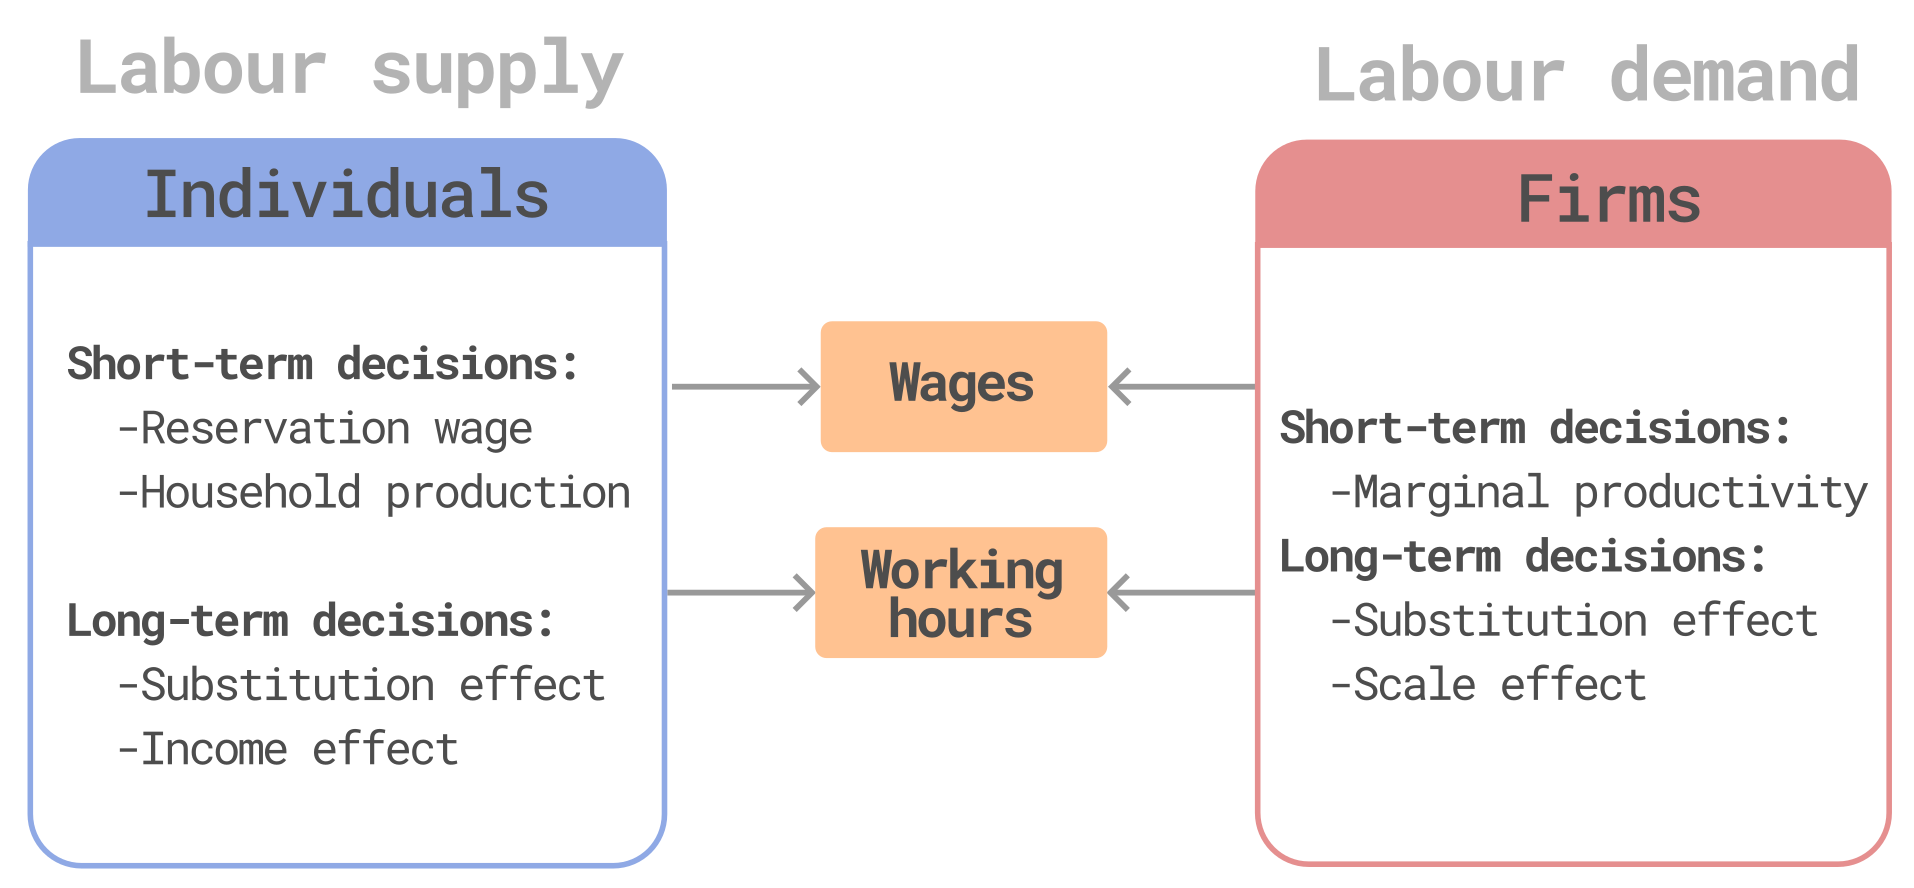
\includegraphics[width=1.0\textwidth]{./images/market_structure.png}
                \captionsetup{labelformat=empty}
                \caption{\fontsize{8pt}{8pt}\selectfont \textbf{\textit{General overview of the Labour market components}}}
            \end{figure}
    \end{columns}
\end{frame}    

\begin{frame}{Modelling labour markets}{Structure}
    \vspace*{-25pt}
    \begin{columns}
        \column{0.4\textwidth}
            \begin{itemize}
                \setlength{\itemsep}{10pt} % Adjust the item separation
                \item \fontsize{10pt}{12pt}\selectfont Labour markets are organized in a \textbf{hierarchical} structure
                \begin{itemize}
                    \item \fontsize{10pt}{12pt}\selectfont Industries
                    \item \fontsize{10pt}{12pt}\selectfont Occupations
                \end{itemize}
                \item \fontsize{10pt}{12pt}\selectfont This structure contributes to the \textbf{wage differentials}.
            \end{itemize}
        \column{0.6\textwidth}
            \begin{figure}
                \centering
                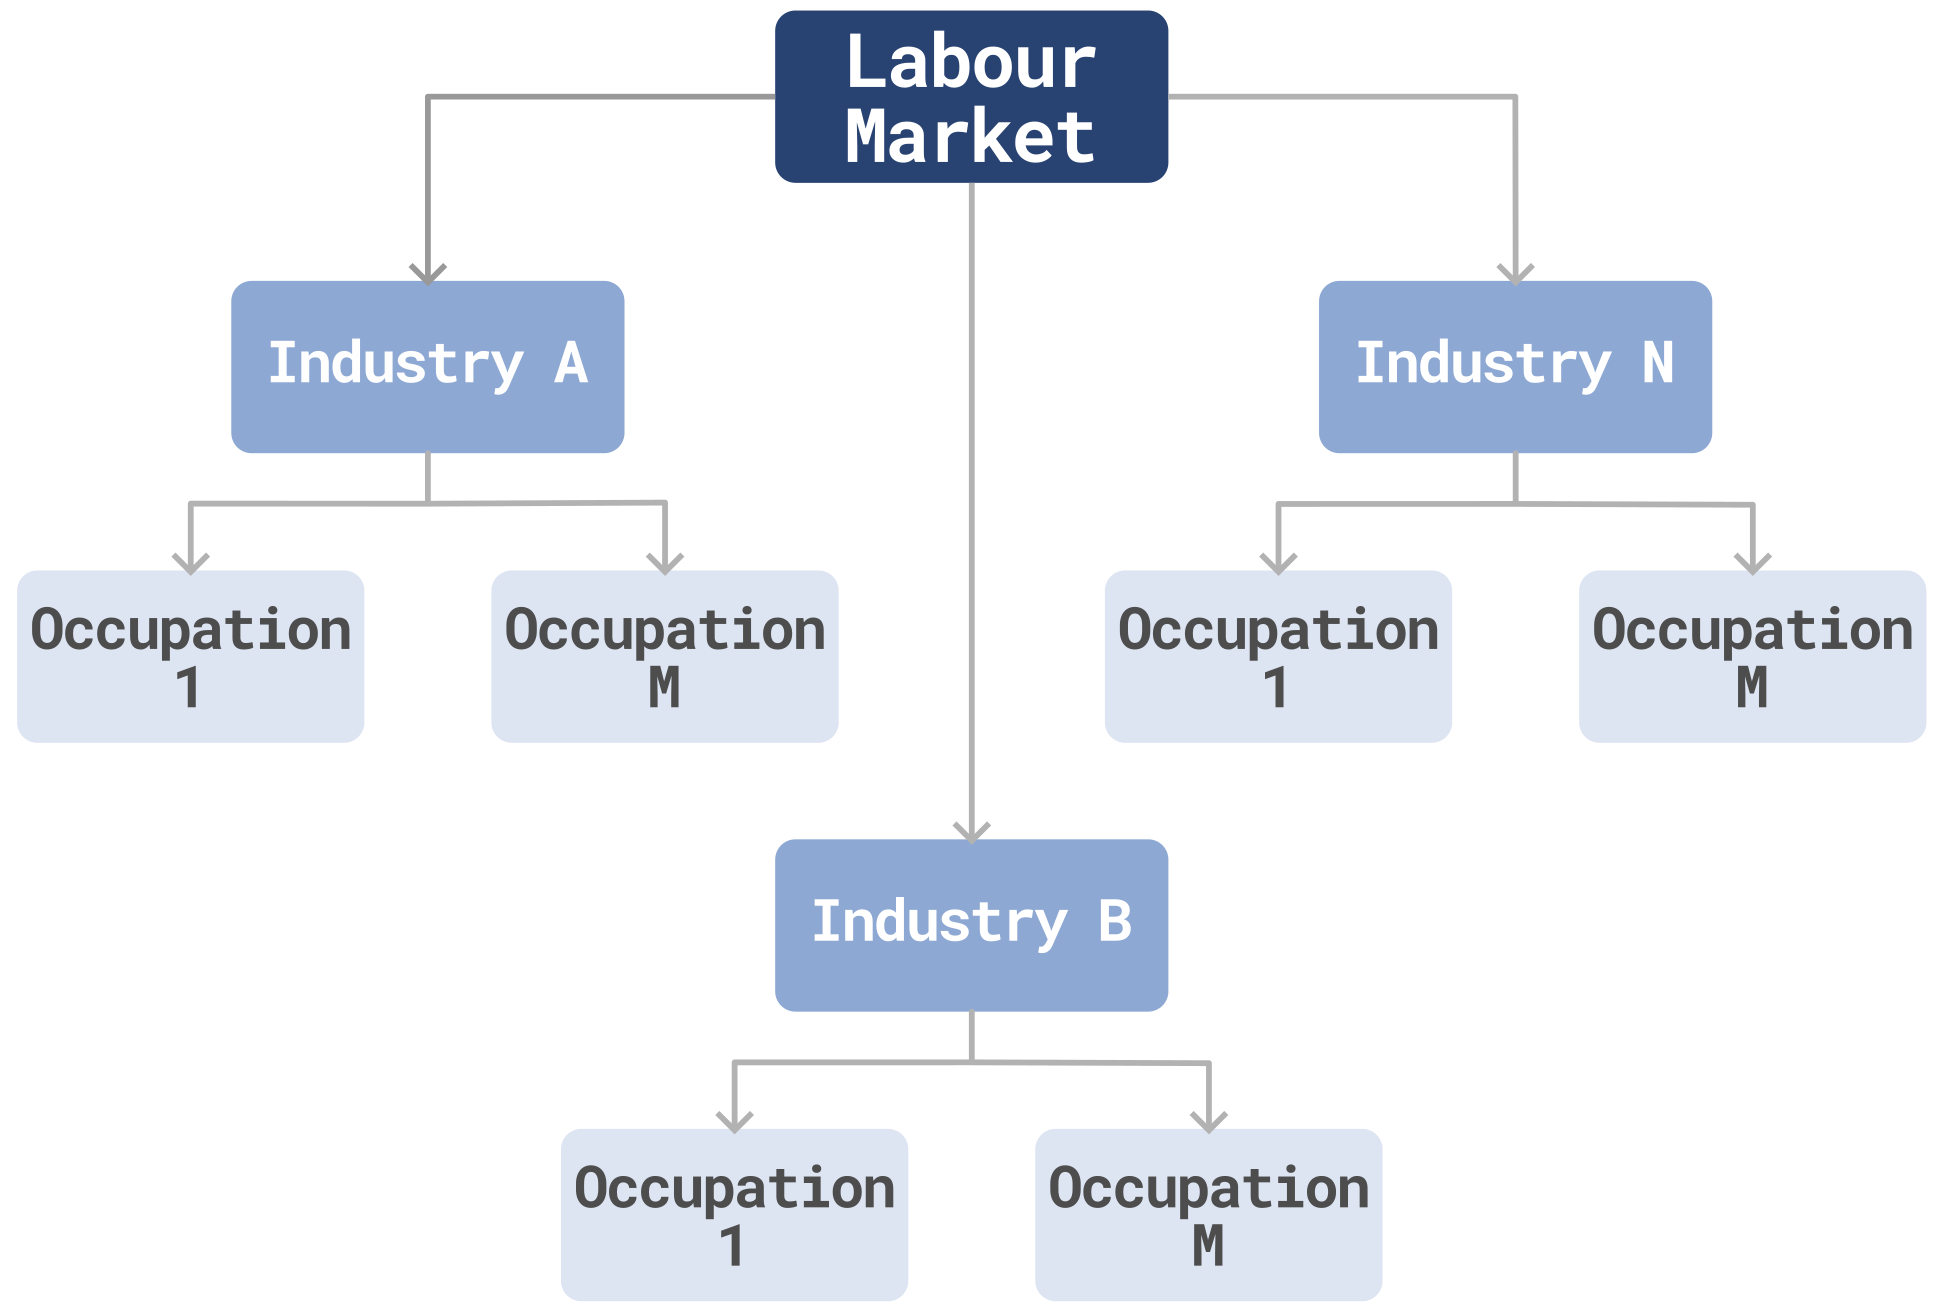
\includegraphics[width=1.0\textwidth]{./images/hierarchical_structure.png}
                \captionsetup{labelformat=empty}
                \caption{\fontsize{8pt}{8pt}\selectfont \textbf{\textit{Hierarchical structure of the labour market}}}
            \end{figure}
    \end{columns}
\end{frame}

\begin{frame}{Modelling labour markets}{ILUTE framework}
    \vspace*{-25pt}
    \begin{columns}
        \column{0.4\textwidth}
            \begin{itemize}
                \setlength{\itemsep}{10pt} % Adjust the item separation
                \item \fontsize{10pt}{12pt}\selectfont Hain (2010) proposed a \textbf{hourly wage model} and a \textbf{transition model}.
                \item \fontsize{10pt}{12pt}\selectfont Harmon (2013) used these models and built an ABM to simulate:
                \begin{itemize}
                    \item \fontsize{10pt}{12pt}\selectfont Worker's state update
                    \item \fontsize{10pt}{12pt}\selectfont Job creation/deletion
                    \item \fontsize{10pt}{12pt}\selectfont Job search and matching
                \end{itemize}
            \end{itemize}
        \column{0.6\textwidth}
            \begin{figure}
                \centering
                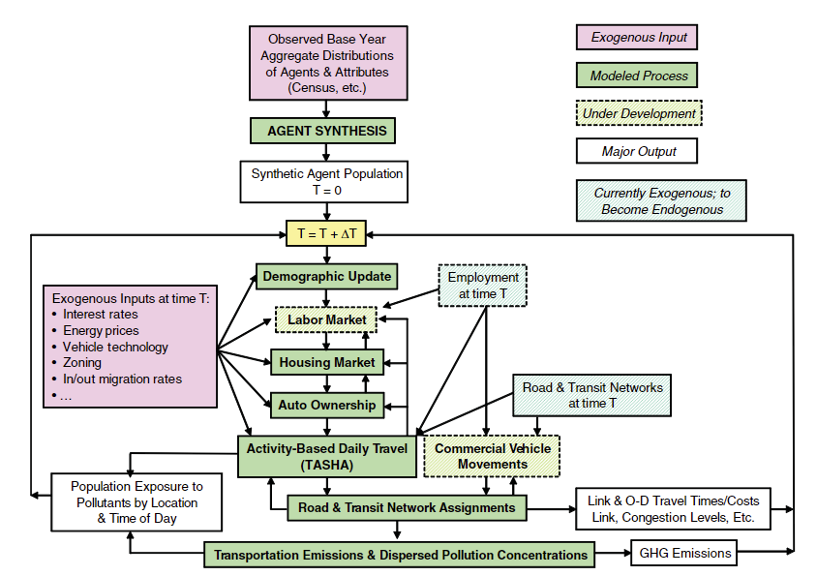
\includegraphics[width=1.0\textwidth]{./images/ilute.png}
                \captionsetup{labelformat=empty}
                \caption{\fontsize{8pt}{8pt}\selectfont \textbf{\textit{ILUTE flowchart (Miller et al, 2021).}}}
            \end{figure}
    \end{columns}
\end{frame}

\begin{frame}{Modelling labour markets}{ILUTE framework}
    \vspace*{-25pt}
    \begin{columns}
        \column{0.5\textwidth}
            \begin{itemize}
                \setlength{\itemsep}{10pt} % Adjust the item separation
                \item \fontsize{10pt}{12pt}\selectfont Harmon (2013) found that:
                \begin{itemize}
                    \item \fontsize{10pt}{12pt}\selectfont The existent wage model is \textbf{underestimating salaries}. 
                    \item \fontsize{10pt}{12pt}\selectfont The source of the problem could be related to the \textbf{Worked Hours} attribute.
                \end{itemize}
            \end{itemize}
            \vspace{15pt}
            \centering
            \textit{The model is missing the random component of the wage distribution (Deterministic vs. Stochastic approach)}
        \column{0.5\textwidth}
            \begin{figure}
                \centering
                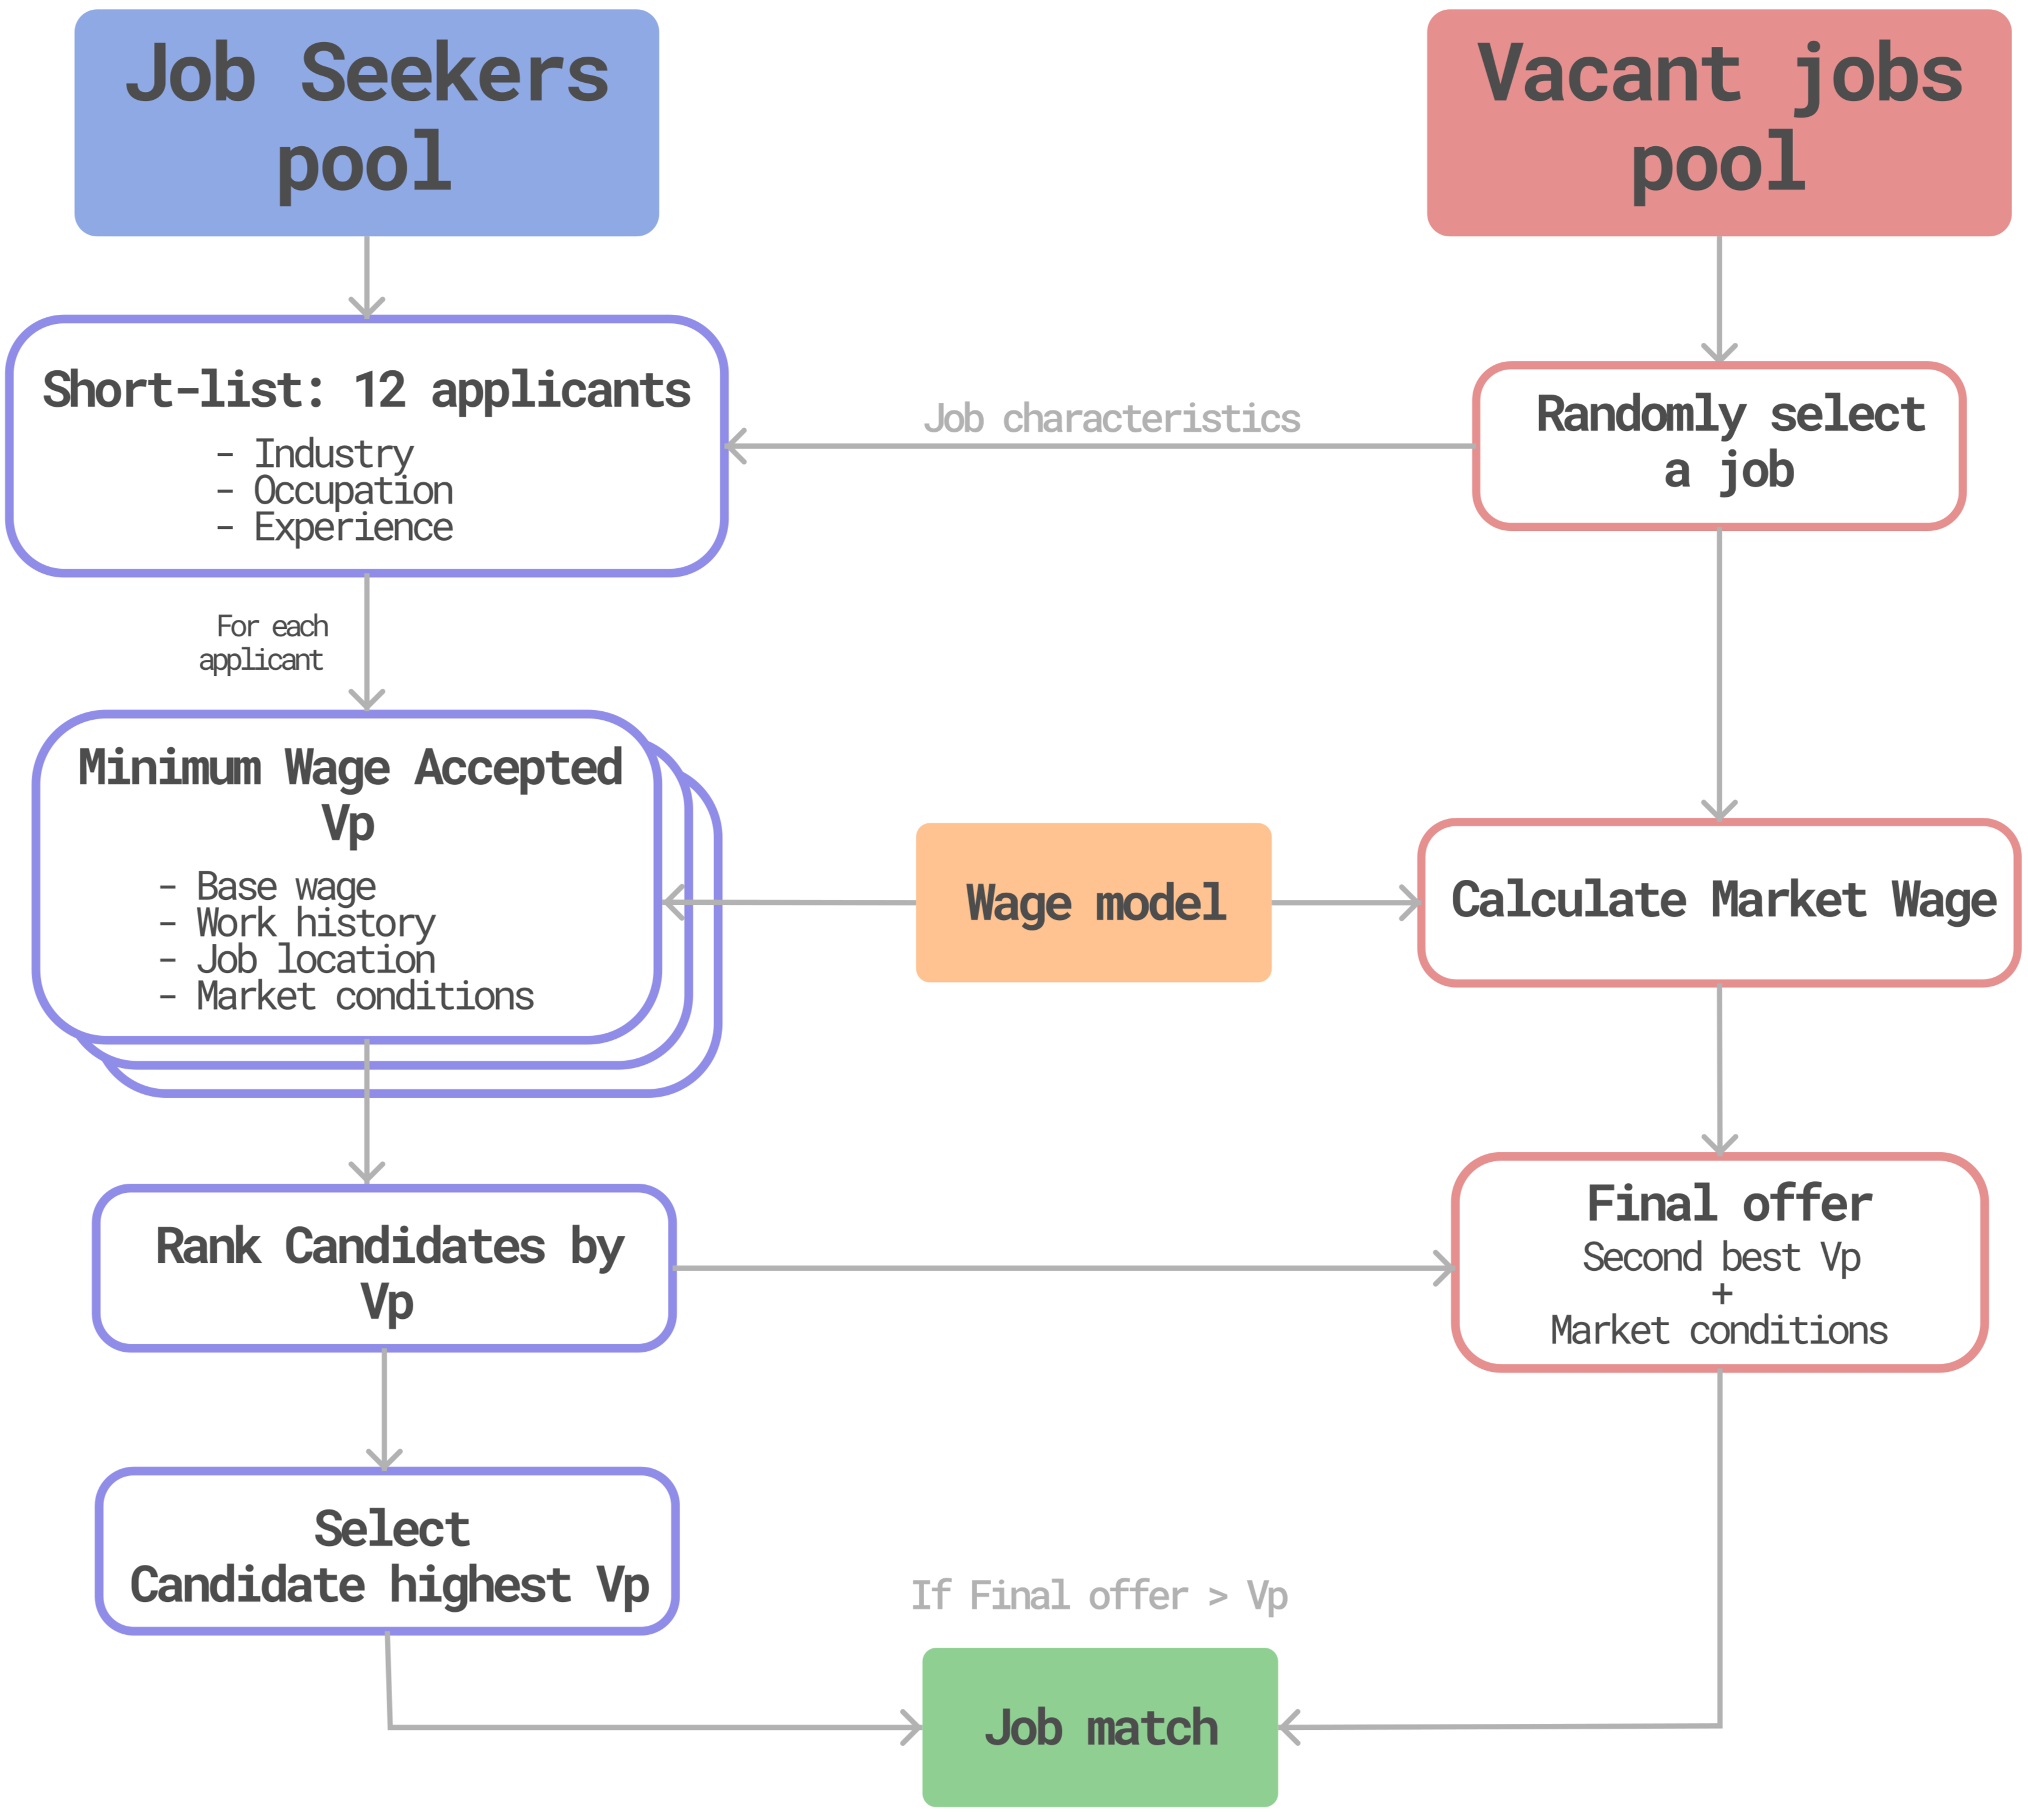
\includegraphics[width=0.9\textwidth]{./images/job_matching.png}
                \captionsetup{labelformat=empty}
                \caption{\fontsize{8pt}{8pt}\selectfont \textbf{\textit{Job search and matching process in ILUTE (Adapted from Harmon,
                2013).}}}
            \end{figure}
    \end{columns}
\end{frame}

{
\setbeamercolor{background canvas}{bg=blue}
\begin{frame}
    \begin{center}
        \textcolor{white}{{\fontsize{22pt}{14pt}\selectfont \textbf{Predicting salaries}}}\\
        \vspace{20pt}
        \textcolor{white}{{\fontsize{14pt}{10pt}\selectfont \textsl{From point estimates to probability distributions}}}
    \end{center}
\end{frame}
}

\begin{frame}{Predicting salaries}{Data sources - SLID Survey}
    \vspace*{-40pt}
    \begin{columns}
        \column{0.6\textwidth}
            \begin{itemize}
                \setlength{\itemsep}{10pt} % Adjust the item separation
                \item \fontsize{10pt}{12pt}\selectfont The \textbf{Survey of Labour and Income Dynamics (SLID) 1996 - 2011}(StatCAN):
                \begin{itemize}
                    \item \fontsize{10pt}{12pt}\selectfont National household survey - Longitudinal 
                    \item \fontsize{10pt}{12pt}\selectfont Panel of ~17K households and 34K respondents
                    \item \fontsize{10pt}{12pt}\selectfont Individuals are interviewed once a year for six years
                \end{itemize}
                \item \fontsize{10pt}{12pt}\selectfont The dataset is split into two sets:
                \begin{itemize}
                    \item \fontsize{10pt}{12pt}\selectfont Training set (1996 - 2007)
                    \item \fontsize{10pt}{12pt}\selectfont Validation set (2008 - 2011)
                \end{itemize}
            \end{itemize}
        \column{0.4\textwidth}
            \begin{figure}
                \centering
                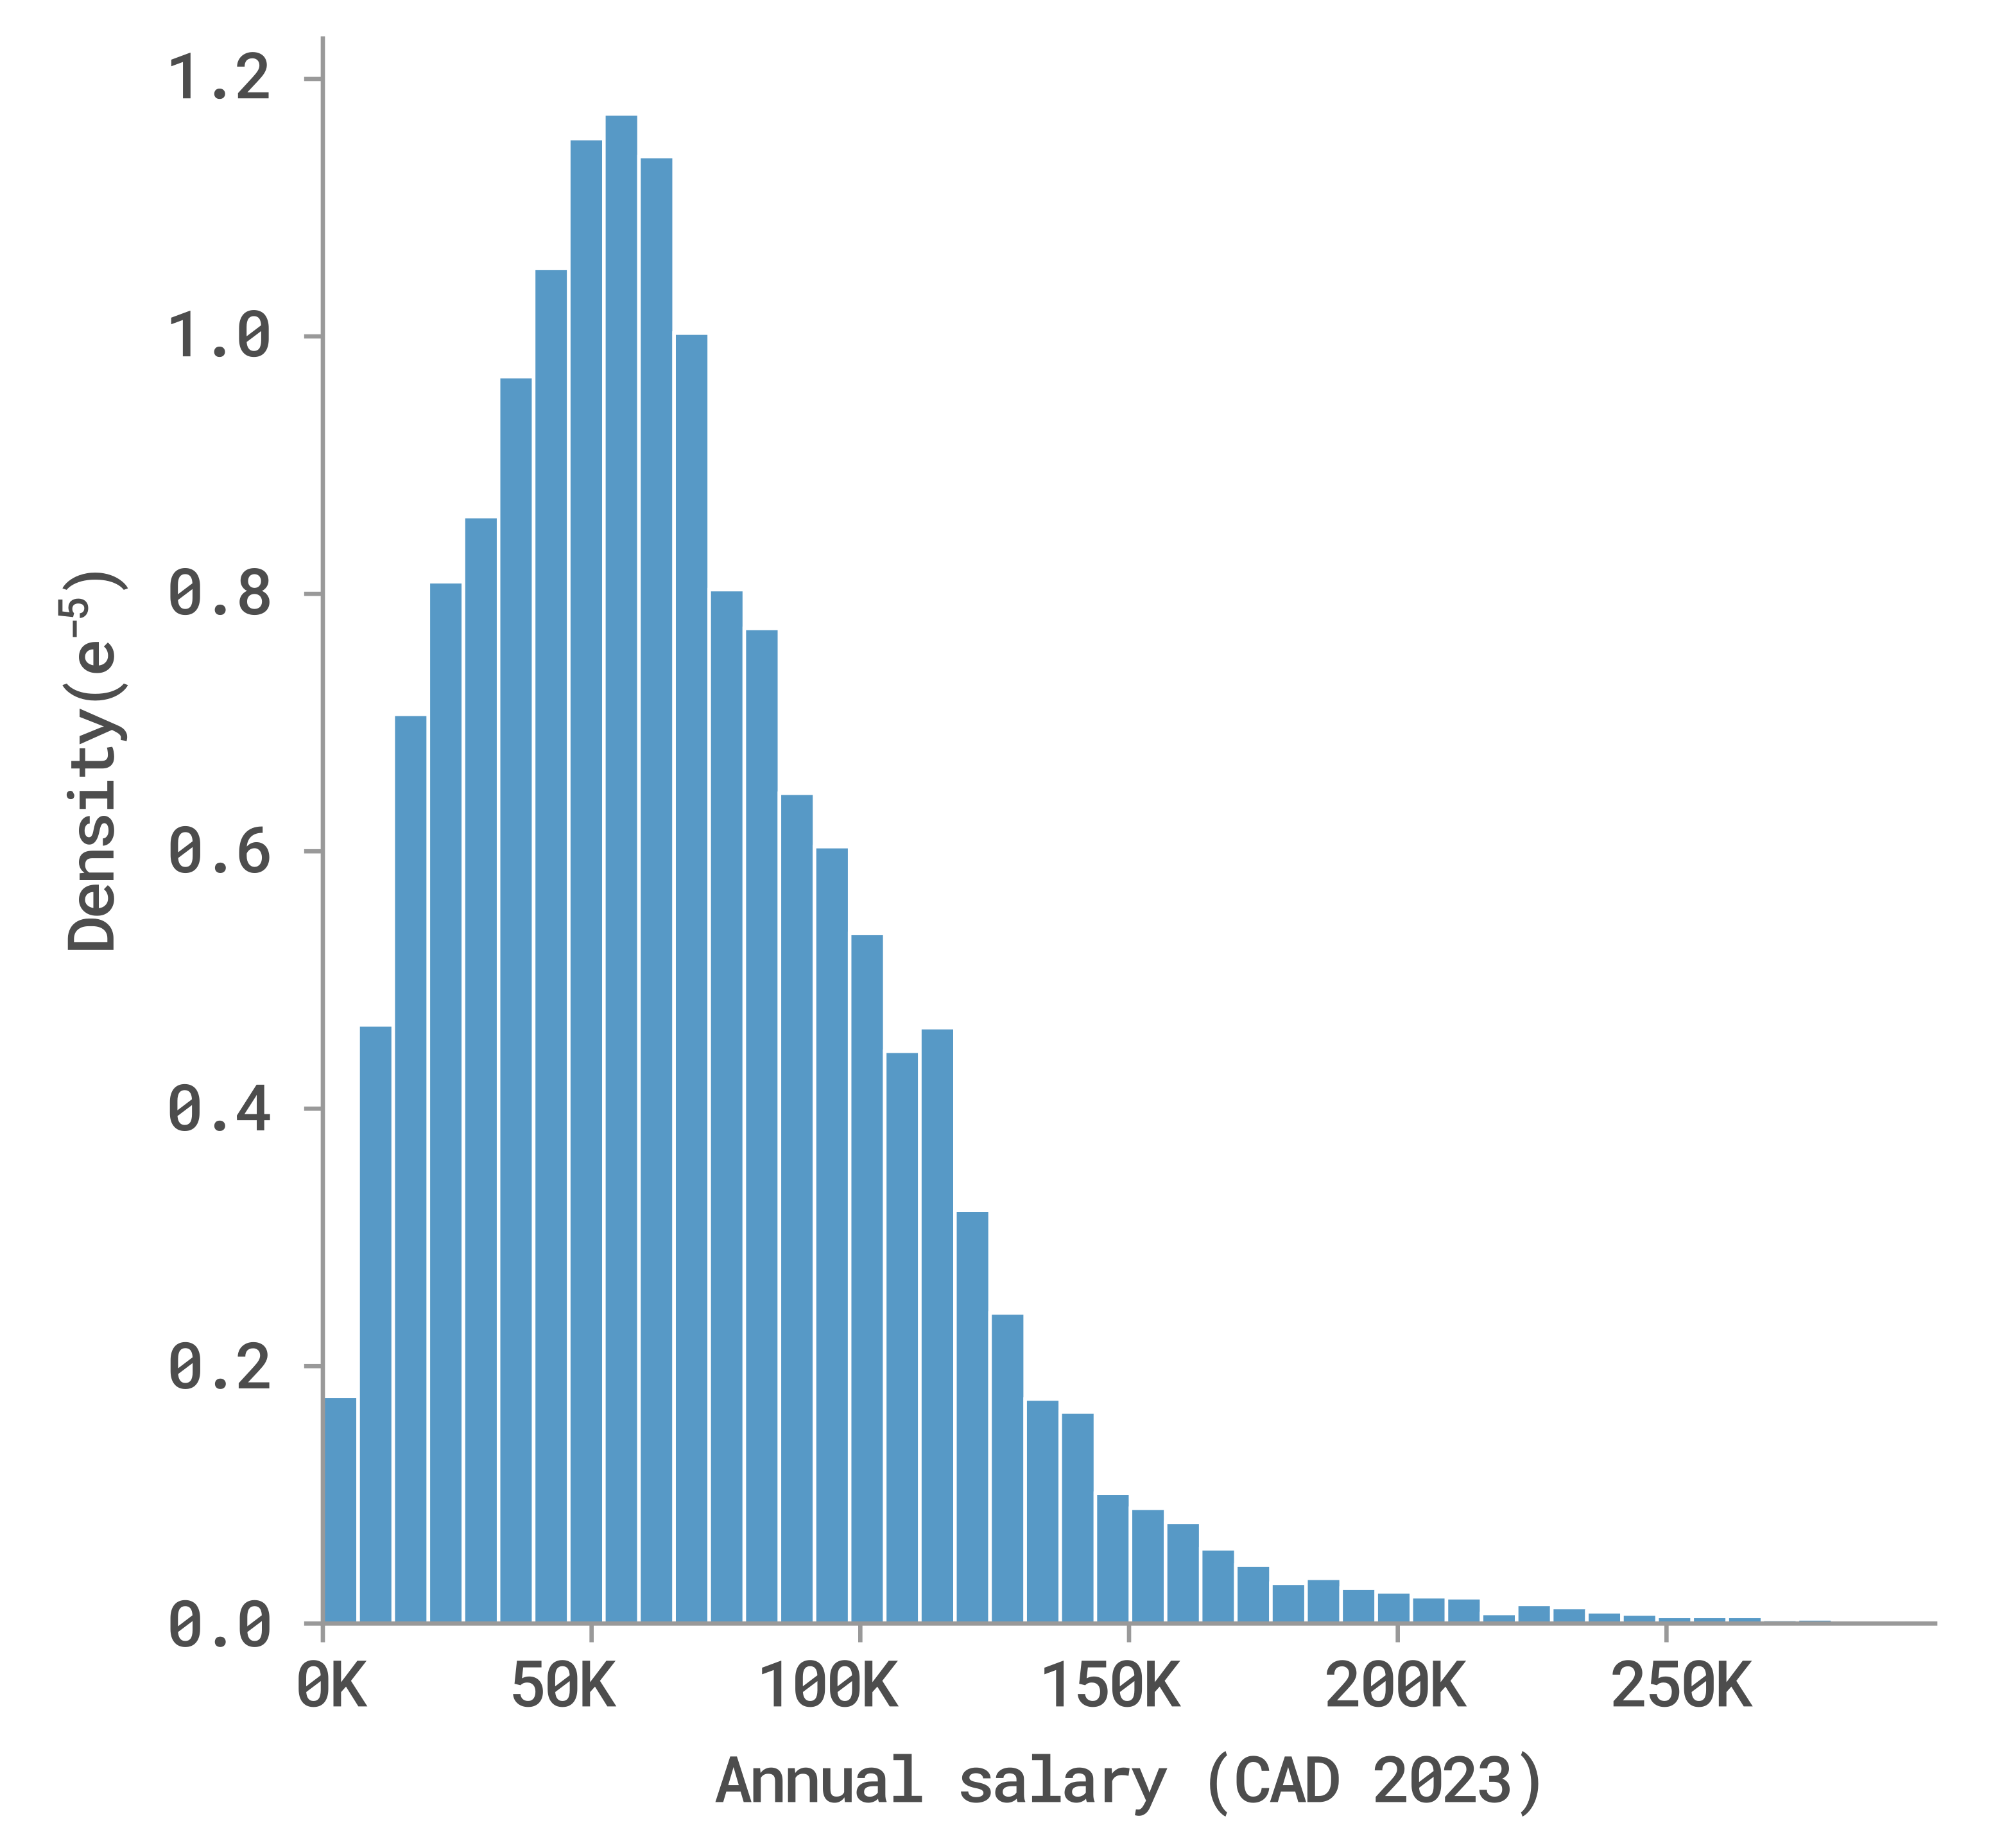
\includegraphics[width=1.0\textwidth]{./images/salary_dist.png}
                \captionsetup{labelformat=empty}
                \setlength{\abovecaptionskip}{-5pt}
                \caption{\fontsize{8pt}{8pt}\selectfont \textbf{\textit{Salary distribution in the GTA 1996-2011}}}
            \end{figure}
        \end{columns}
    \centering \textit{*Salary data is converted to real terms (CAD 2023) using the CPI.}
\end{frame}

\begin{frame}{Predicting salaries}{Exploratory Data Analysis}
    \vspace*{-80pt}
    \begin{columns}
        \column{0.41\textwidth}
            \begin{itemize}
                \setlength{\itemsep}{10pt} % Adjust the item separation
                \item \fontsize{10pt}{12pt}\selectfont Age, experience, and tenure are \textbf{positively correlated} with salaries.
                \item \fontsize{10pt}{12pt}\selectfont Weak linear relationship with \textbf{high variance}.
            \end{itemize}
        \column{0.59\textwidth}
            \begin{figure}
                \centering
                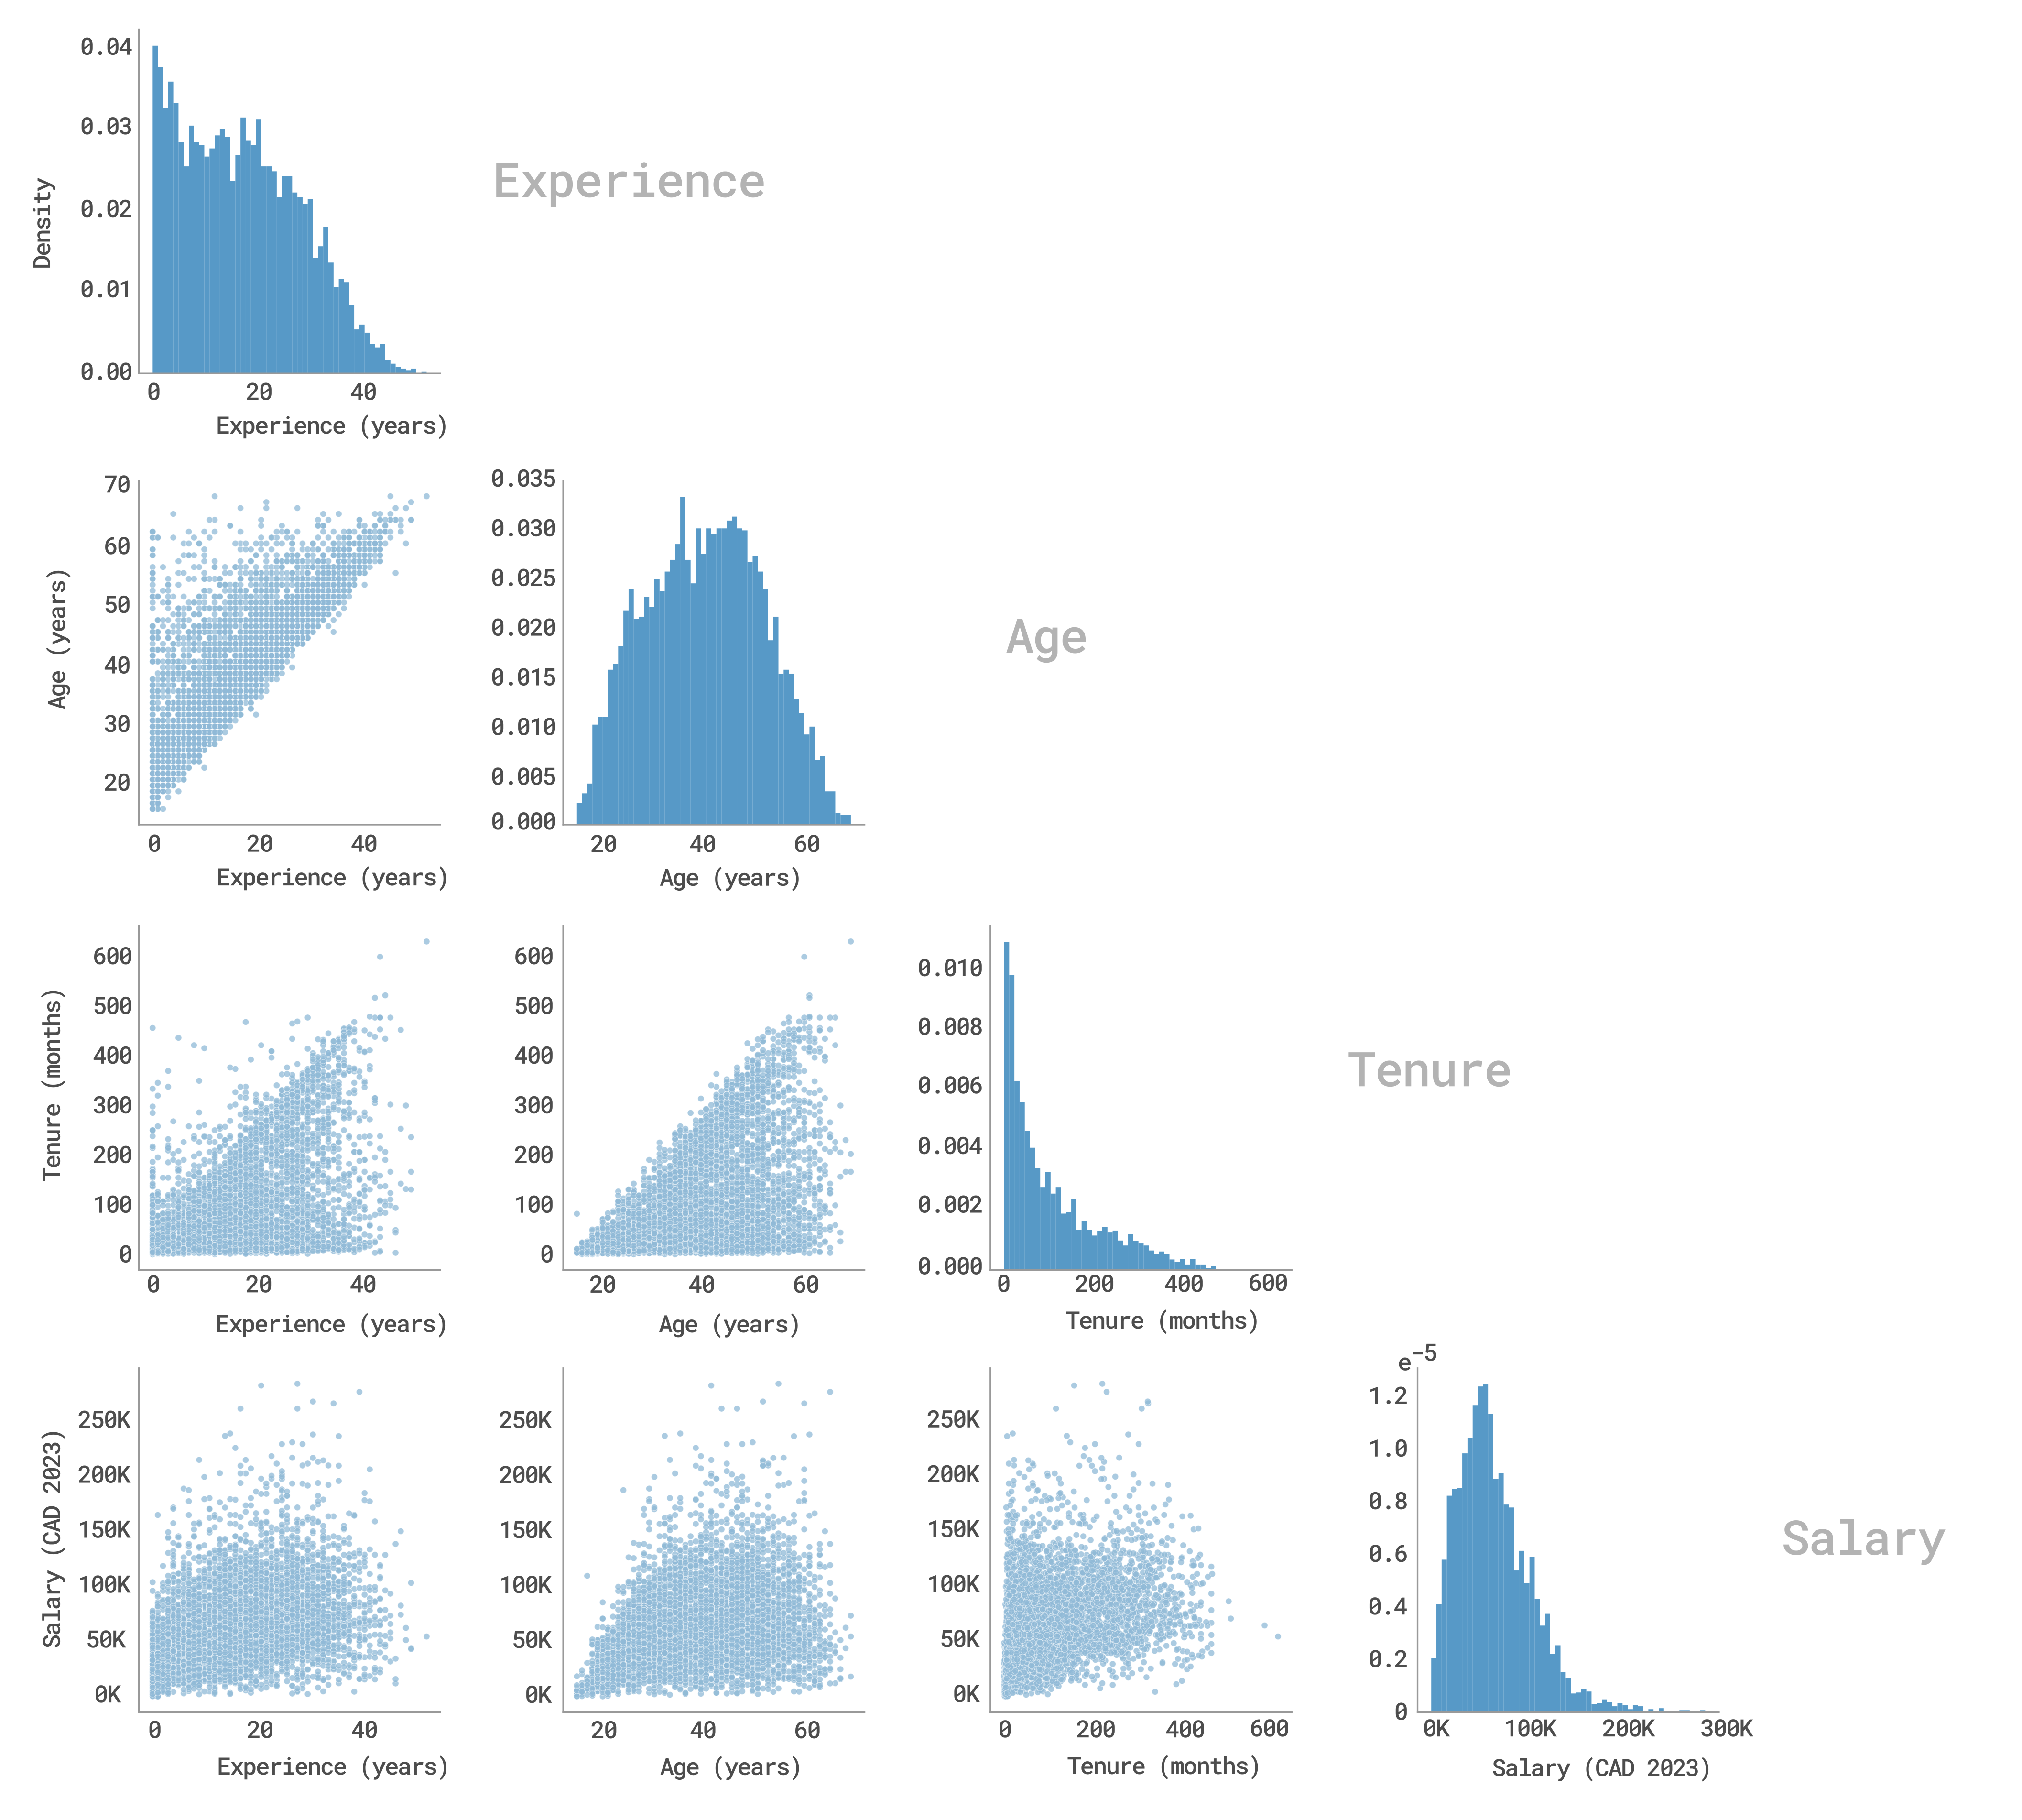
\includegraphics[width=1.1\textwidth]{./images/pairplot.png}
                \captionsetup{labelformat=empty}
                \setlength{\abovecaptionskip}{-16pt}
                \caption{\fontsize{8pt}{8pt}\selectfont \textbf{\textit{Salaries by experience, age, and tenure in the GTA 1996-2011}}}
            \end{figure}
    \end{columns}
\end{frame} 

\begin{frame}{Predicting salaries}{Exploratory Data Analysis}
    \vspace*{-30pt}
    \begin{figure}
        \centering
        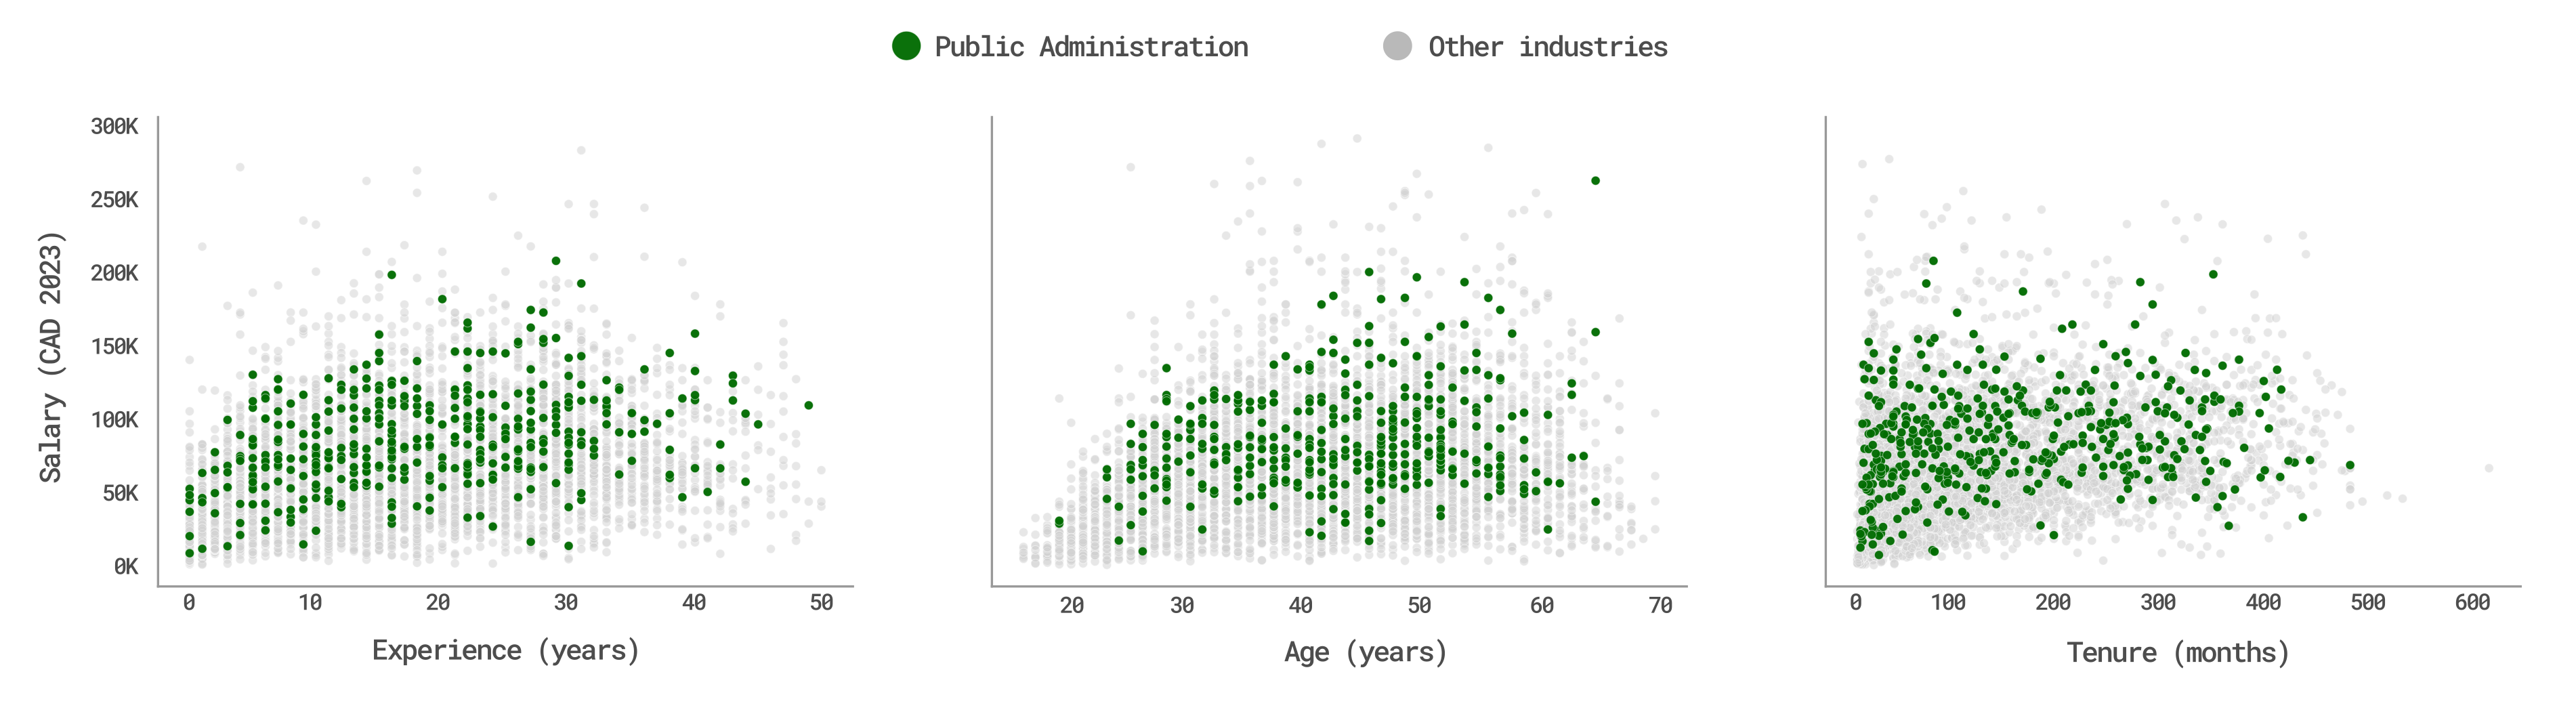
\includegraphics[width=1.0\textwidth]{./images/eda_salary_ind.png}
        \captionsetup{labelformat=empty}
        \setlength{\abovecaptionskip}{-10pt}
        \caption{\fontsize{8pt}{8pt}\selectfont \textbf{\textit{Salaries by experience, age, and tenure for Public Admin in the GTA 1996-2011}}}
    \end{figure}
    \centering \textit{Given the hierarchical structure, the linear relationship between some predictors becomes more explicit when data is filtered by industry and occupation}
\end{frame} 

\begin{frame}{Predicting salaries}{Model structure}
    \vspace*{-16pt}
    \begin{figure}
        \centering
        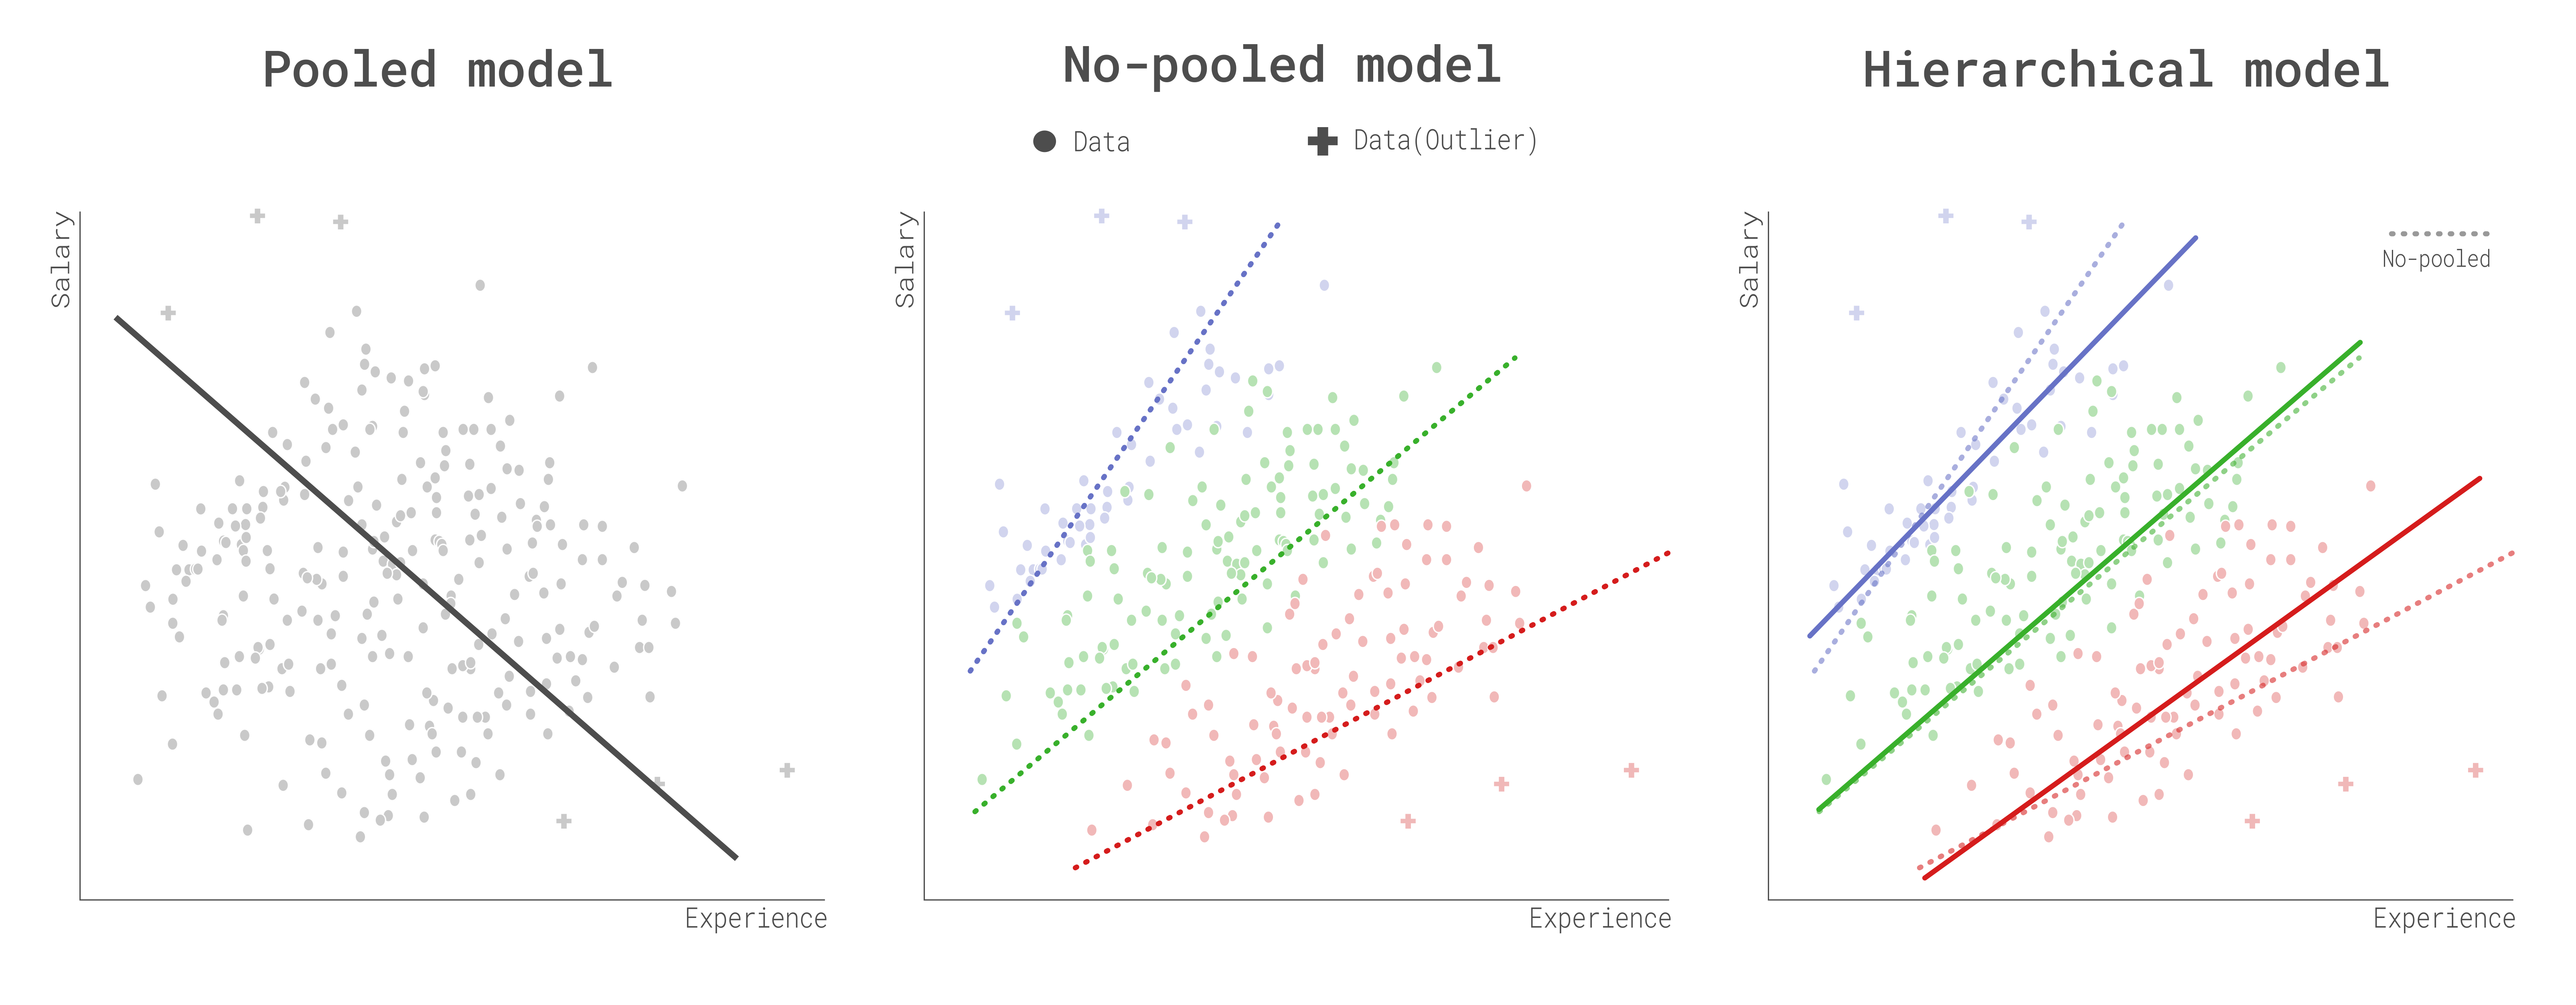
\includegraphics[width=0.8\textwidth]{./images/simpsons_paradox.png}
        \captionsetup{labelformat=empty}
        \setlength{\abovecaptionskip}{-7pt}
        \caption{\fontsize{8pt}{8pt}\selectfont \textbf{\textit{Effect of model structure on the data representation}}}
    \end{figure}
    \centering \textit{The Hierarchical model catptures the \textbf{data heterogeneity}, is more \textbf{robust to outliers}, and reduces the \textbf{risk of overfitting}.}
\end{frame}

\begin{frame}{Predicting salaries}{Model structure - Pooled}
    \vspace*{-30pt}
    \begin{columns}
        \column{0.5\textwidth}
            \begin{figure}
                \centering
                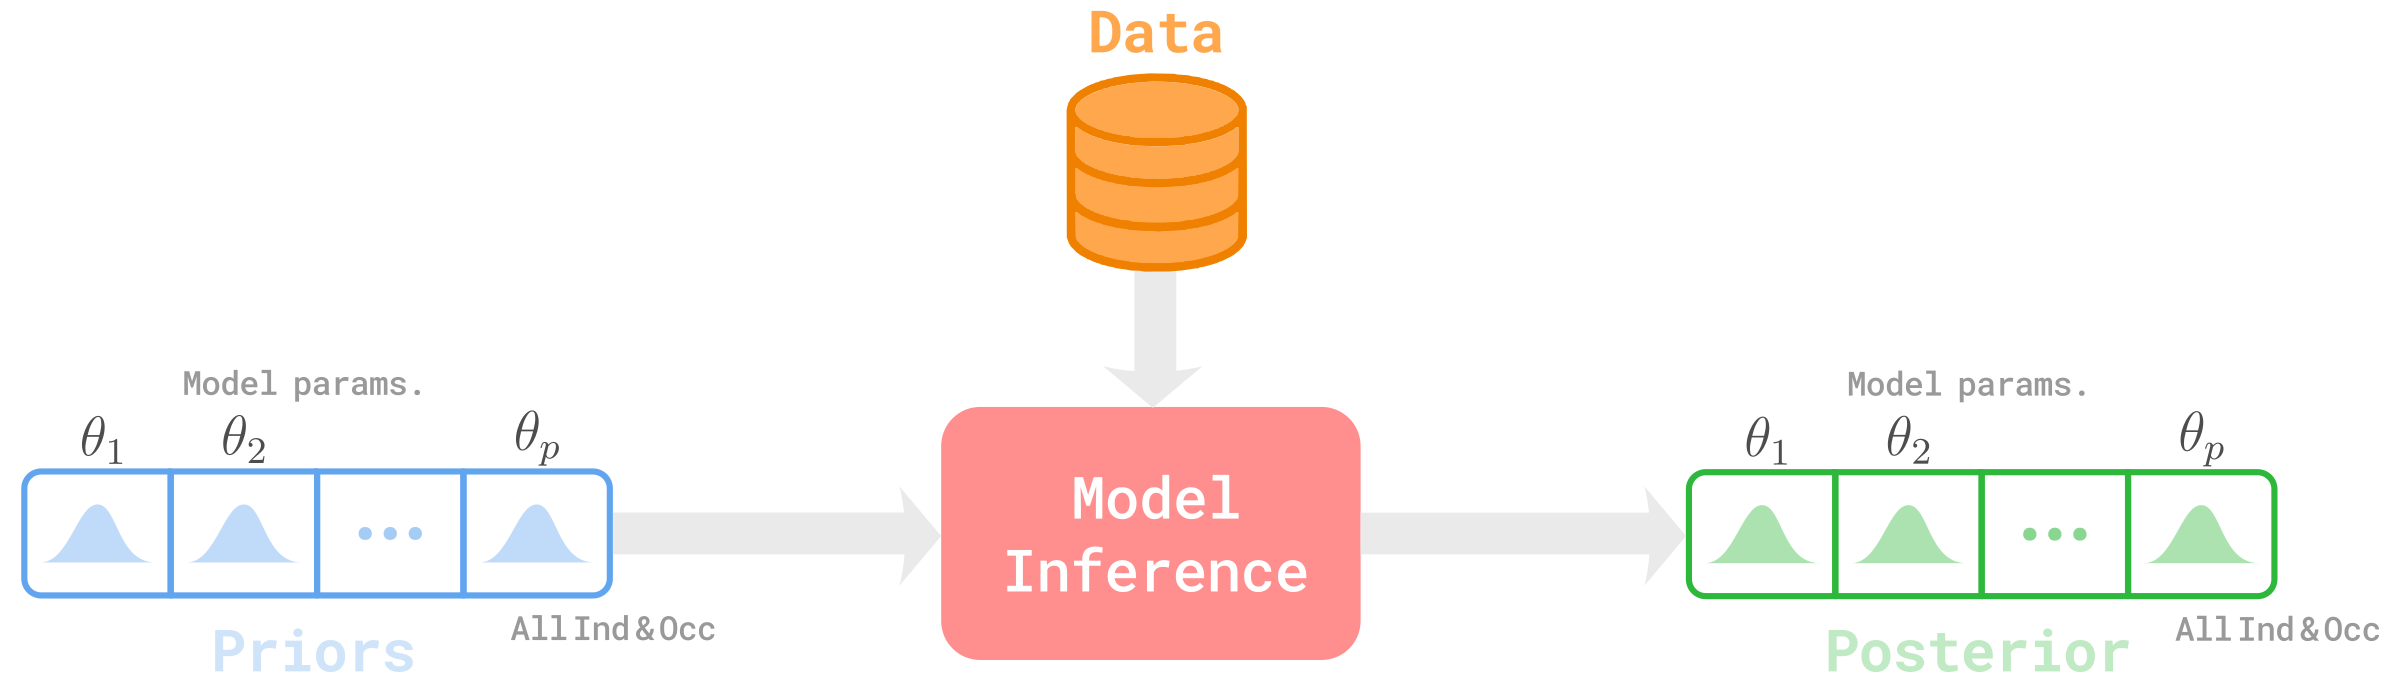
\includegraphics[width=1.0\textwidth]{./images/pooled.png}
                \captionsetup{labelformat=empty}
                \setlength{\abovecaptionskip}{-5pt}
                \caption{\fontsize{8pt}{8pt}\selectfont \textbf{\textit{Bayesian inference for the pooled model}}}
            \end{figure}
        \column{0.5\textwidth}
            \begin{figure}
                \centering
                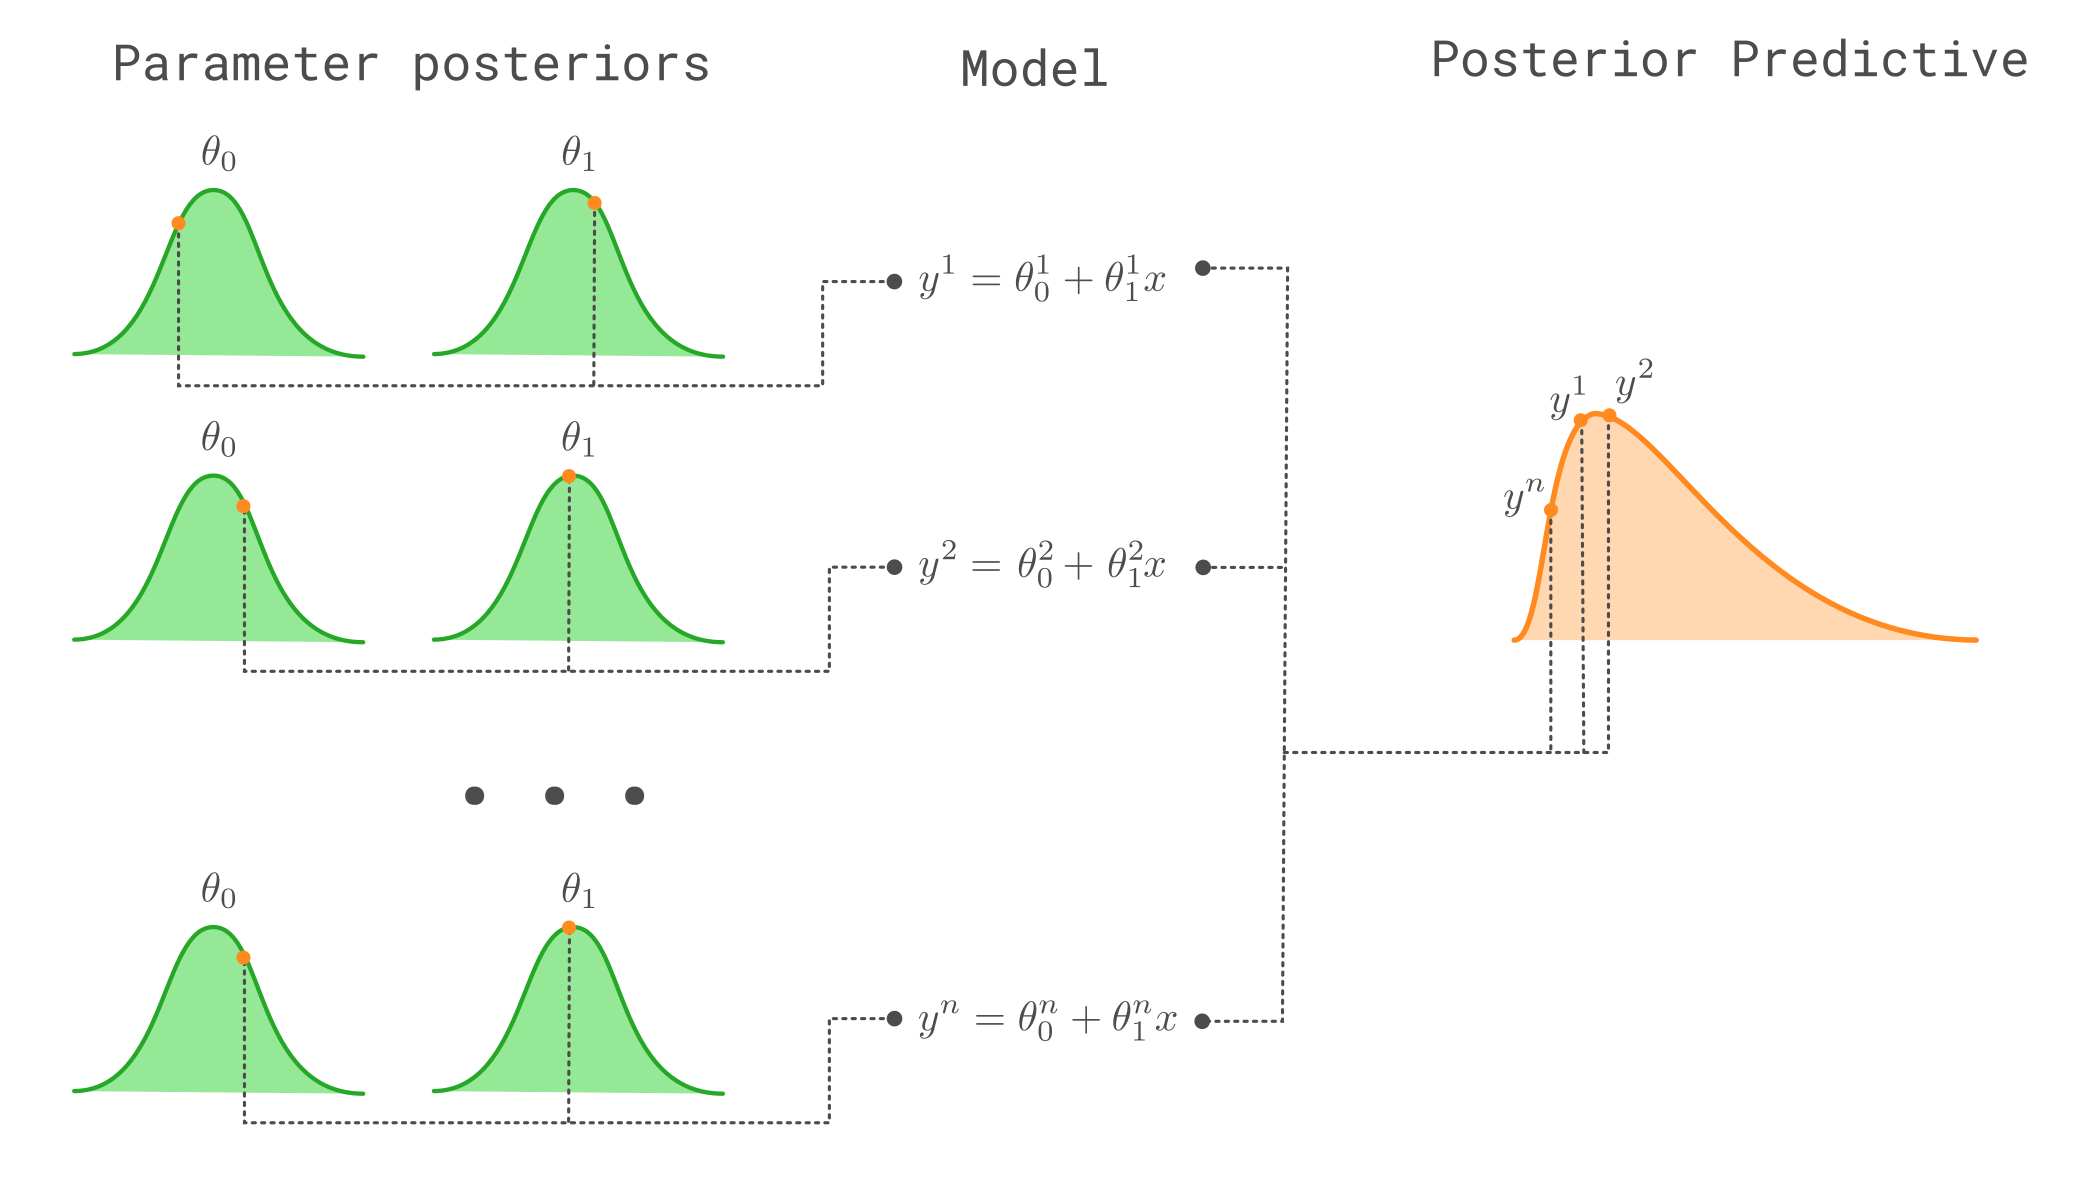
\includegraphics[width=1.0\textwidth]{./images/posterior_pred.png}
                \captionsetup{labelformat=empty}
                \setlength{\abovecaptionskip}{-5pt}
                \caption{\fontsize{8pt}{8pt}\selectfont \textbf{\textit{Predictions using the posterior distributions}}}
            \end{figure}
    \end{columns}
\end{frame}

\begin{frame}{Predicting salaries}{Model structure - No-Pooled}
    \begin{figure}
        \centering
        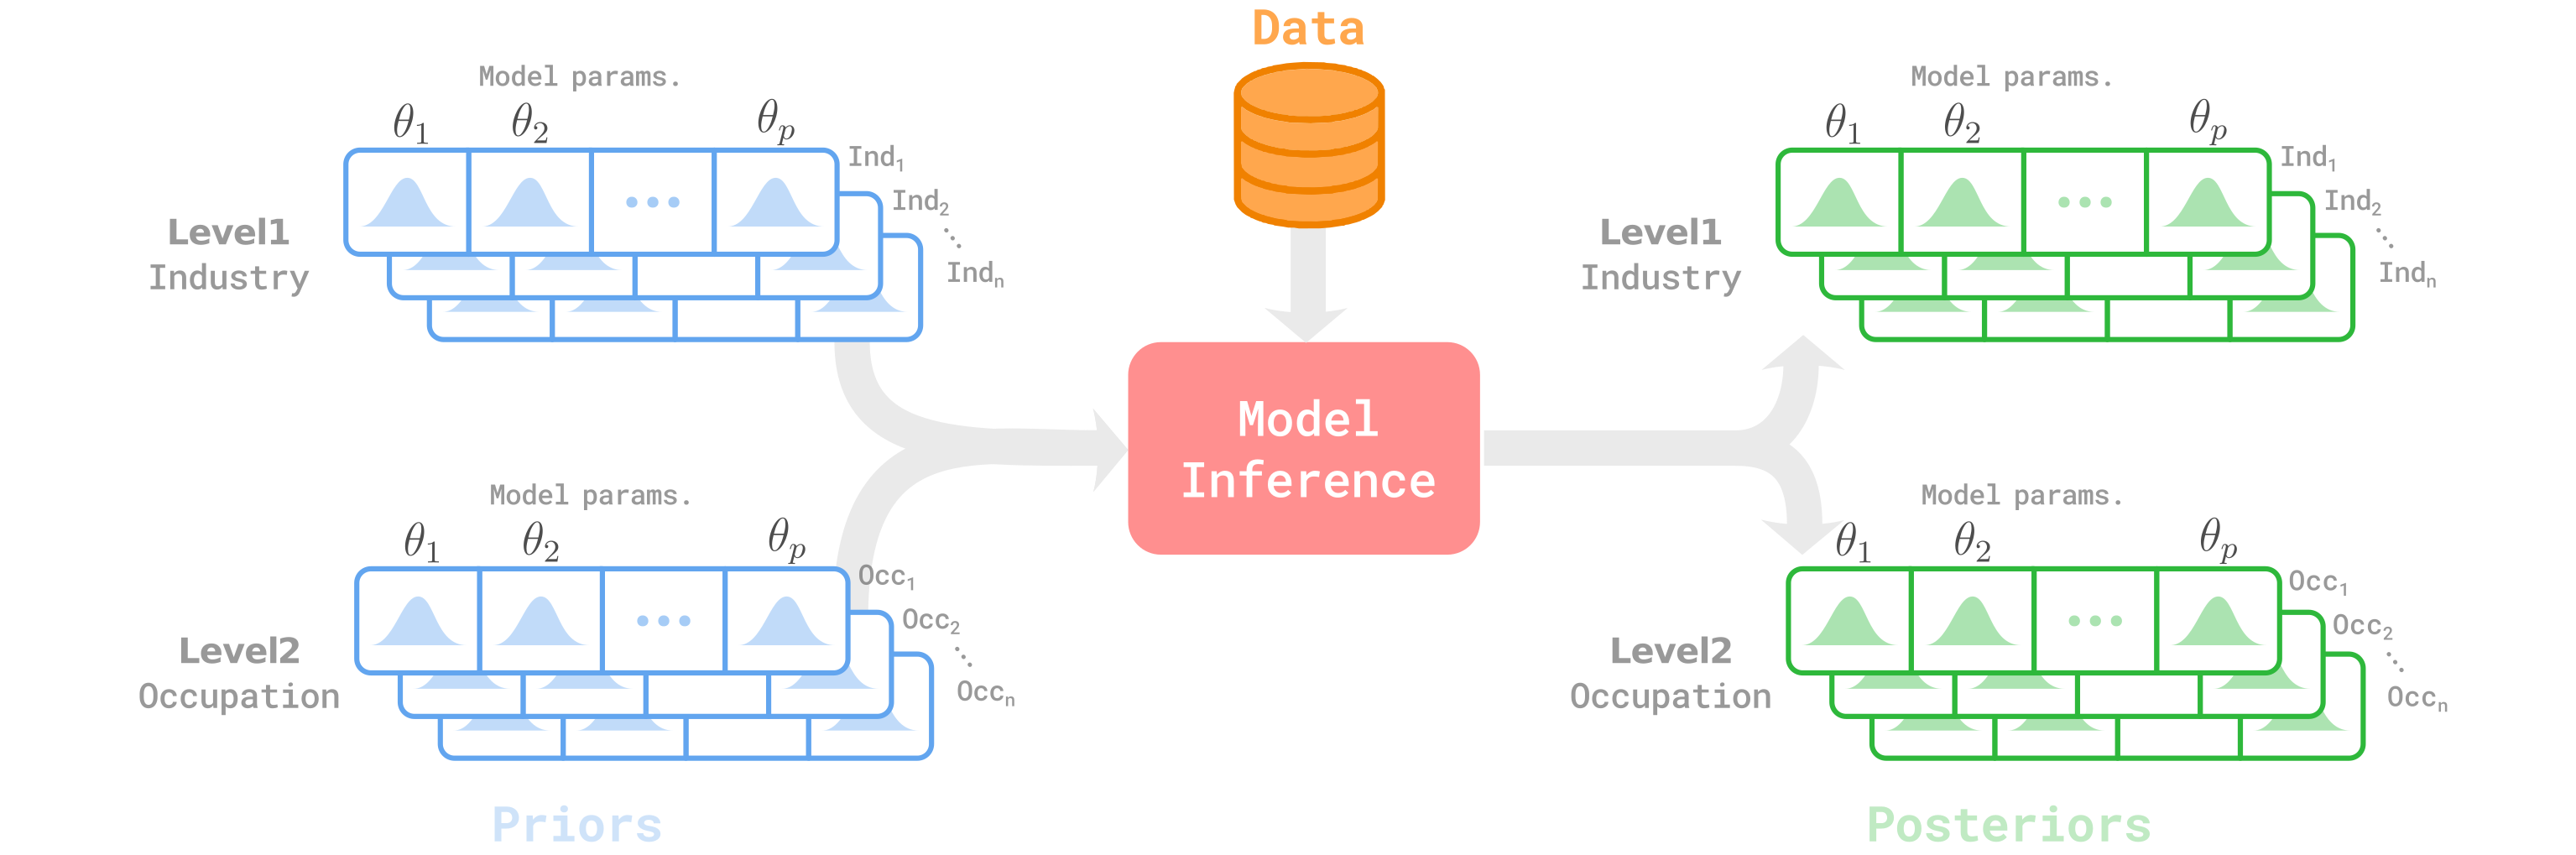
\includegraphics[width=1.0\textwidth]{./images/no-pooled.png}
        \captionsetup{labelformat=empty}
        \setlength{\abovecaptionskip}{-5pt}
        \caption{\fontsize{8pt}{8pt}\selectfont \textbf{\textit{Bayesian inference for the no-pooled model}}}
    \end{figure}
\end{frame}

\begin{frame}{Predicting salaries}{Model structure - Hierarchical}
    \vspace*{-16pt}
    \begin{figure}
        \centering
        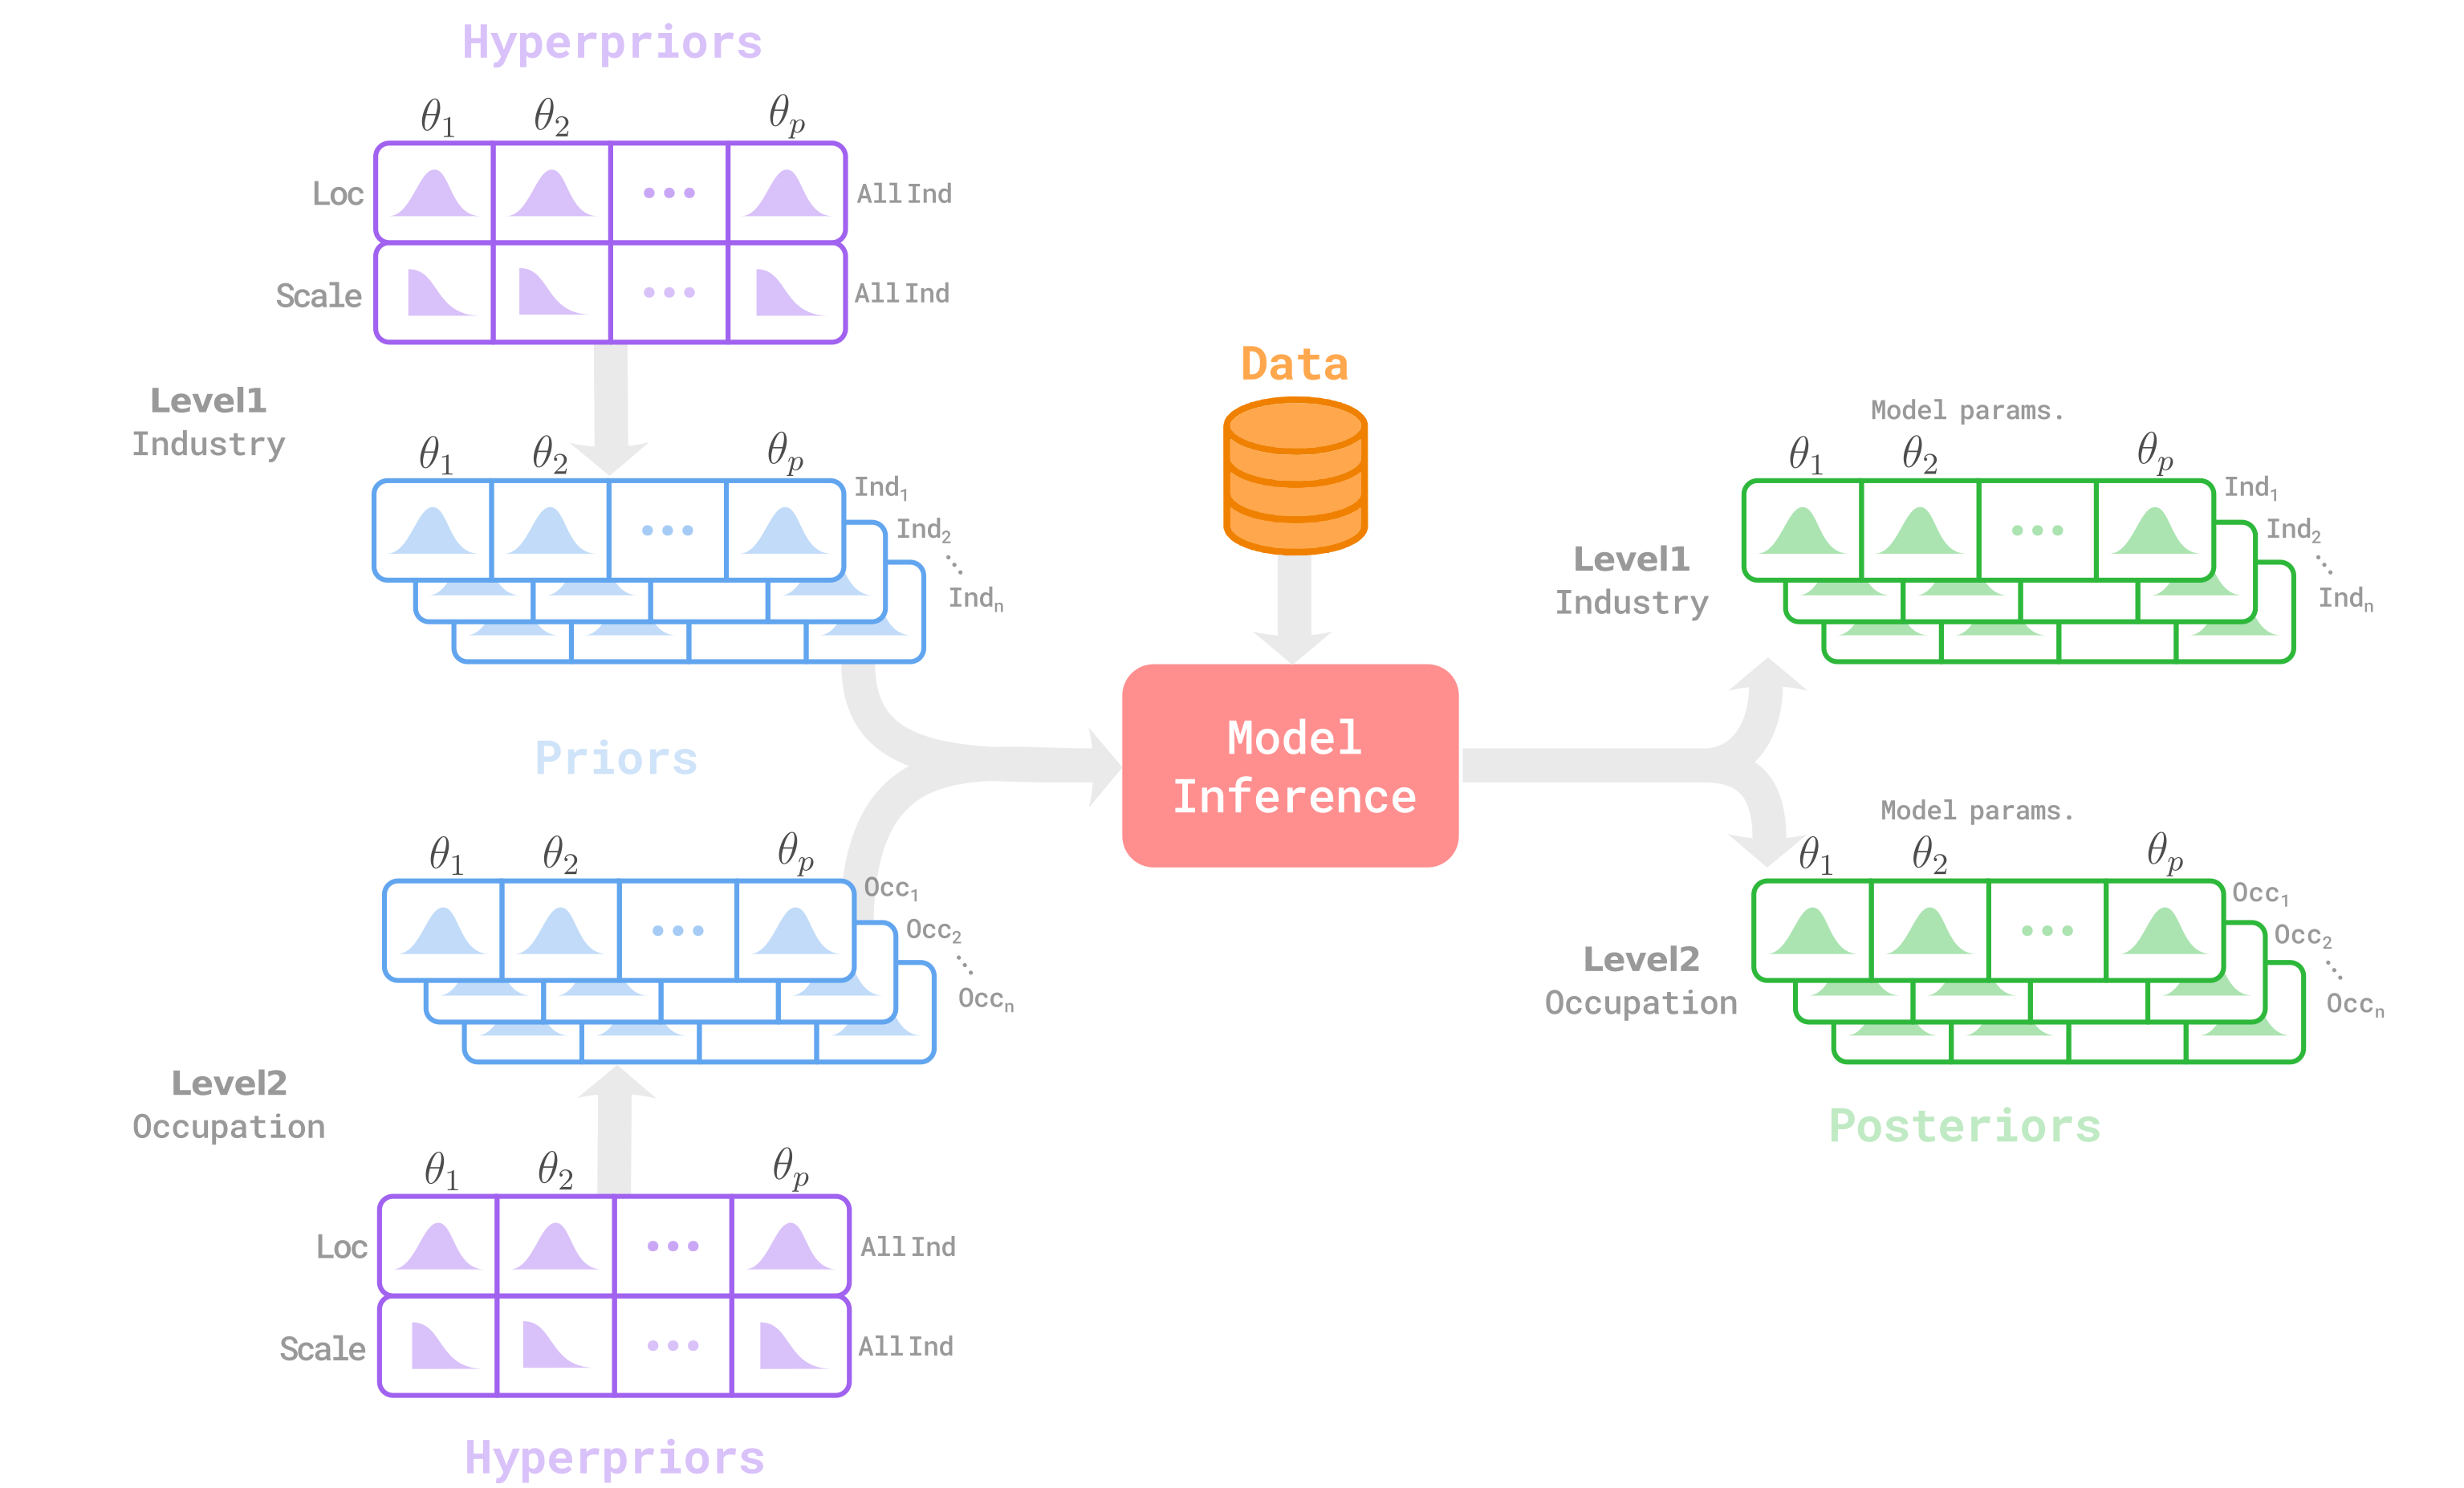
\includegraphics[width=0.7\textwidth]{./images/hierarchical.png}
        \captionsetup{labelformat=empty}
        \caption{\fontsize{8pt}{8pt}\selectfont \textbf{\textit{Bayesian inference for the hierarchical model}}}
    \end{figure}
\end{frame}

\begin{frame}{Predicting salaries}{Model specification}
    \begin{columns}
        \column{0.4\textwidth}
            \vspace*{-20pt}
            {\tiny\begin{align*}
                \eqnmarkbox[lightPurple]{hyperprior}{loc_{p}^{ind} \sim Normal(0,1)}\\[-5pt]\nonumber
                \eqnmarkbox[lightPurple]{hyperprior}{scale_{p}^{ind} \sim HalfNormal(1)}\\[-5pt]\nonumber
                \eqnmarkbox[lightPurple]{hyperprior}{loc_{p}^{occ} \sim Normal(0,1)}\\[-5pt]\nonumber
                \eqnmarkbox[lightPurple]{hyperprior}{scale_{p}^{occ} \sim HalfNormal(1)}\\\nonumber
                \eqnmarkbox[lightBlue]{prior}{\alpha\sim Uniform(0, 100)}\\[-5pt]\nonumber
                \eqnmarkbox[lightBlue]{prior}{\theta_{p}^{ind} \sim Normal(loc_{p}^{ind}, scale_{p}^{ind})}\\[-5pt]\nonumber
                \eqnmarkbox[lightBlue]{prior}{\theta_{p}^{occ} \sim Normal(loc_{p}^{occ}, scale_{p}^{occ})}\\\nonumber
                \eqnmarkbox[lightGrey]{calculation}{\eta^{ind} = \theta_0^{ind}+\theta_1^{ind}X_1+...+\theta_p^{ind}X_p}\\[-5pt]\nonumber
                \eqnmarkbox[lightGrey]{calculation}{\eta^{occ} = \theta_0^{occ}+\theta_1^{occ}X_1+...+\theta_p^{occ}X_p}\\[-5pt]\nonumber
                \eqnmarkbox[lightGrey]{calculation}{\mu=e^{\eta^{ind}+\eta^{occ}}}\\[-5pt]\nonumber
                \eqnmarkbox[lightGrey]{calculation}{\beta=\alpha/\mu}\\\nonumber
                \eqnmarkbox[lightGreen]{posterior}{Y \sim} \eqnmarkbox[lightRed]{random}{Gamma(\alpha,\beta)}\\\nonumber         
            \end{align*}}
        \column{0.6\textwidth}
            \vspace*{-80pt}
            \begin{figure}
                \centering
                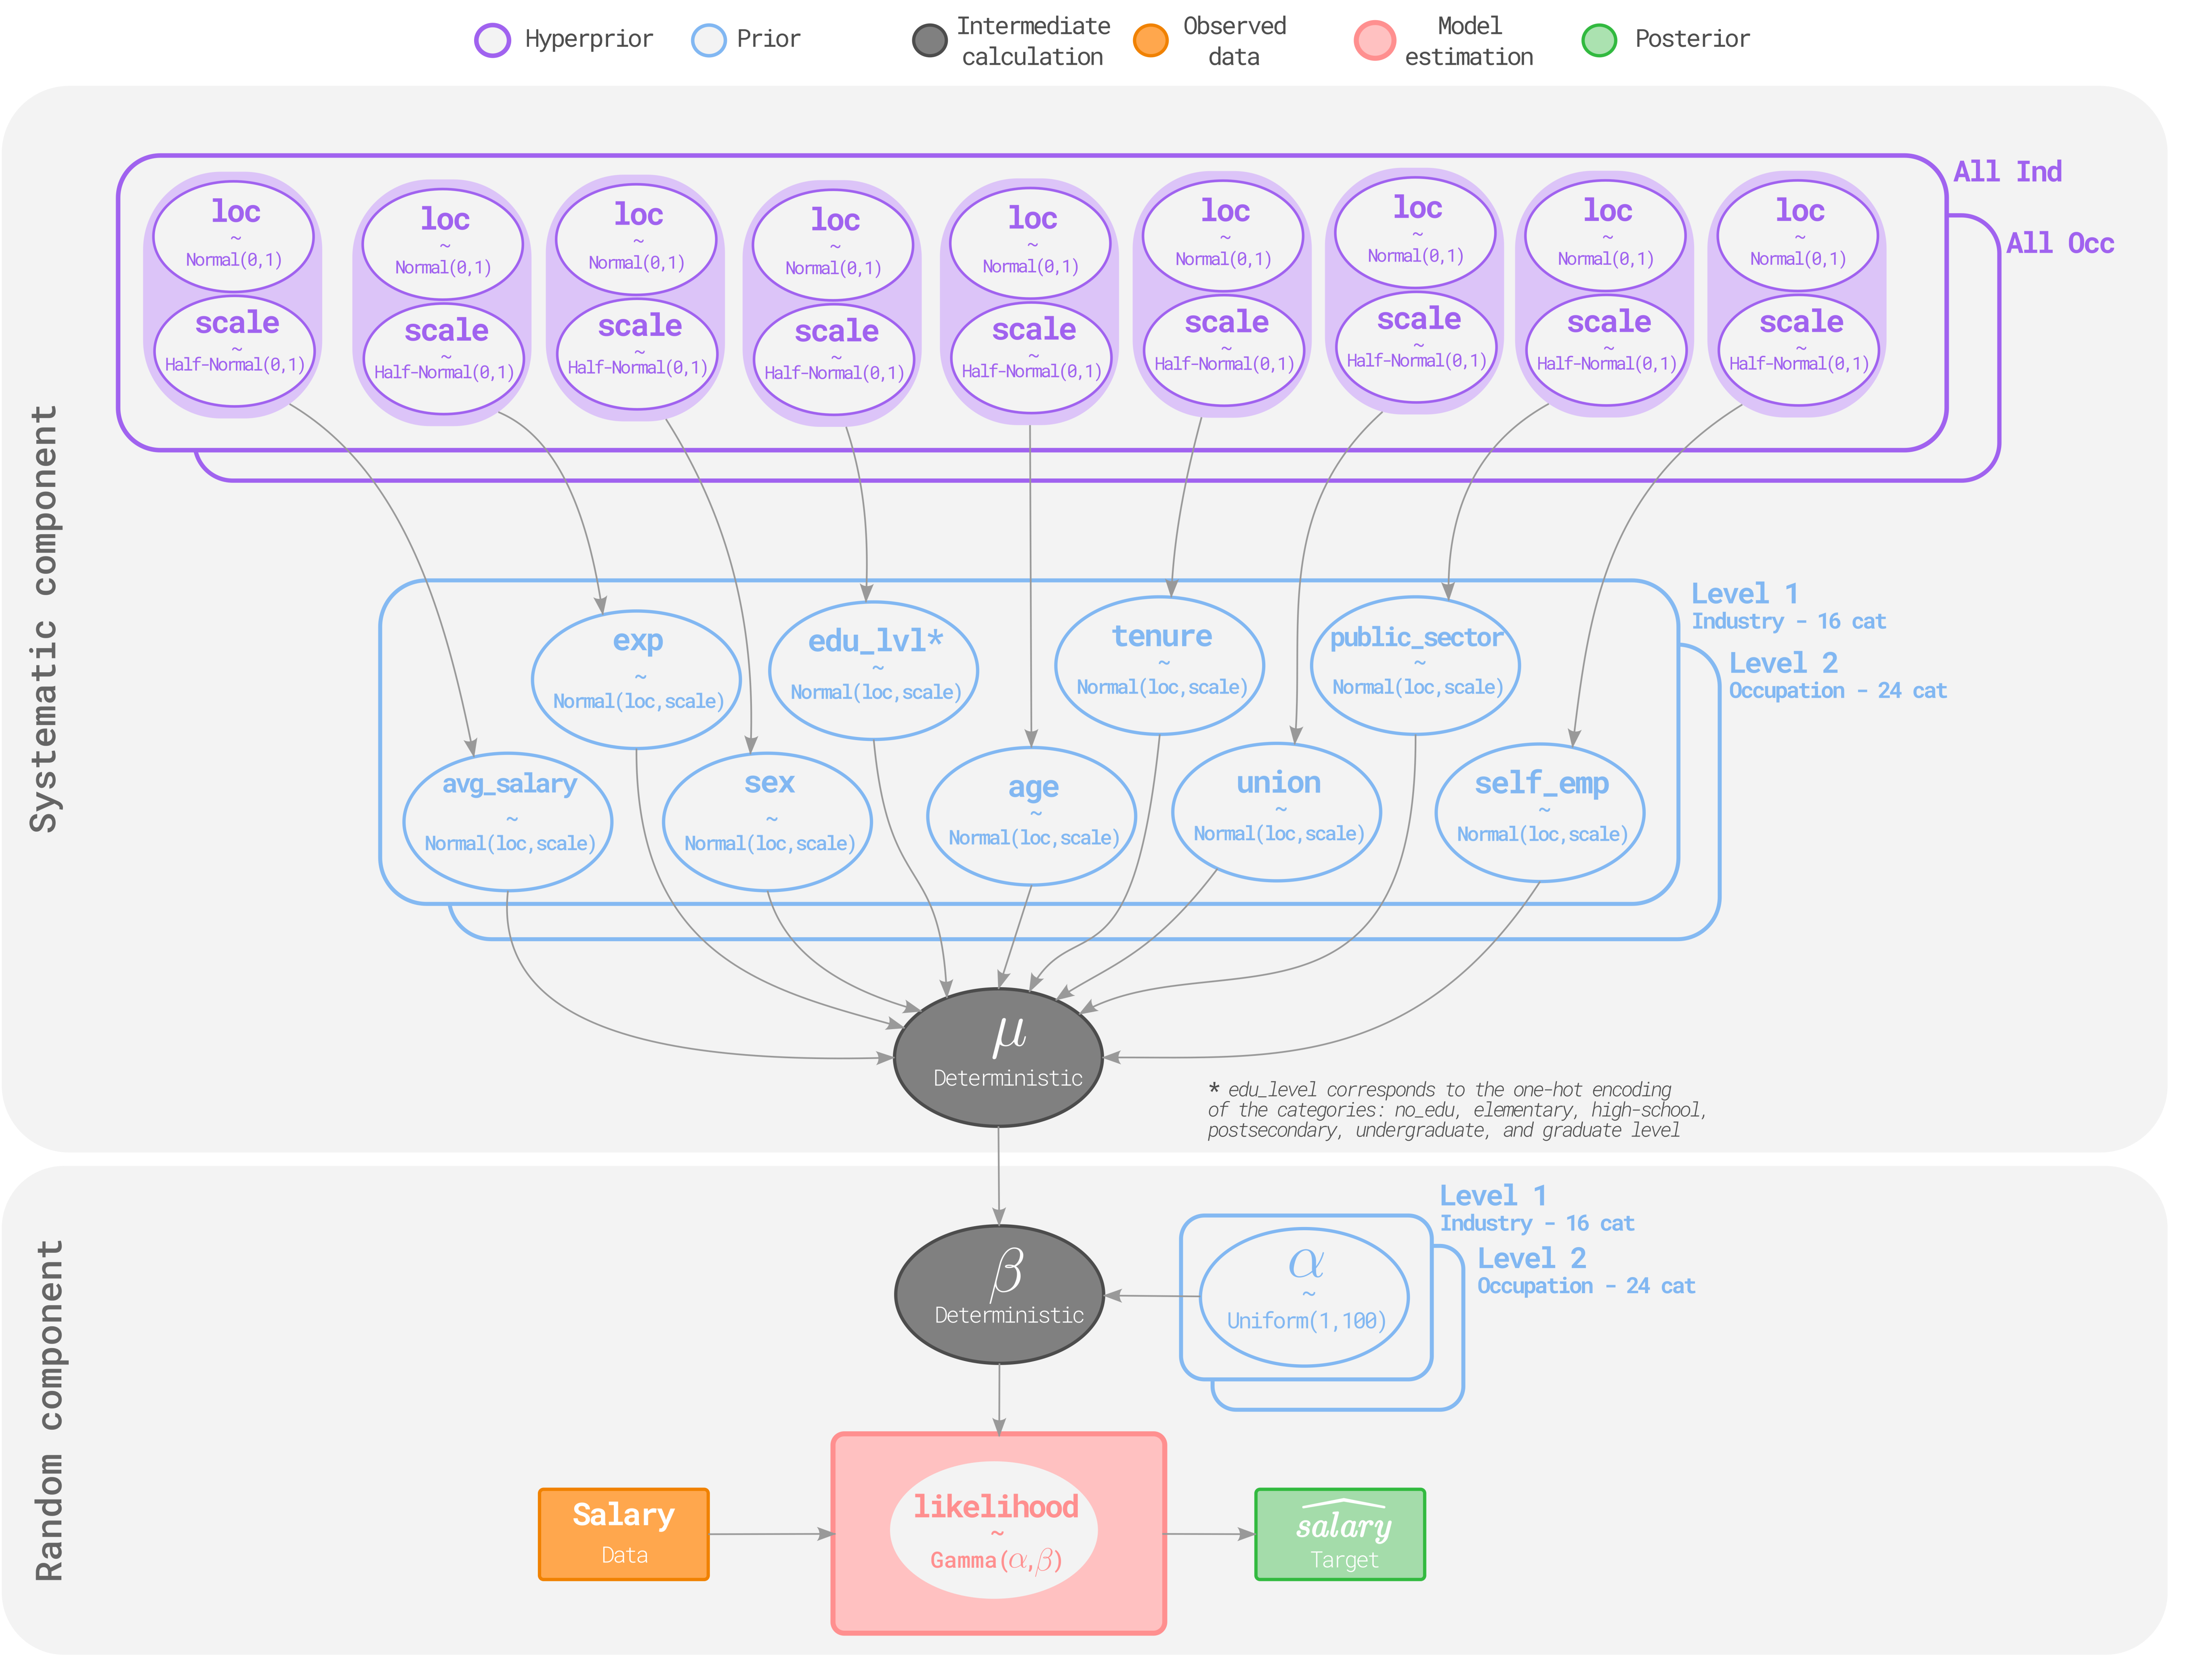
\includegraphics[width=1.07\textwidth]{./images/hierarchical_graph.png}
                \captionsetup{labelformat=empty}
                \setlength{\abovecaptionskip}{-10pt}
                \caption{\fontsize{8pt}{8pt}\selectfont \textbf{\textit{Hierarchical model graph}}}
            \end{figure}
    \end{columns}
\end{frame}

\begin{frame}{Predicting salaries}{Model specification - Results}
    \vspace*{-20pt}
    \begin{columns}
        \column{0.4\textwidth}
            \begin{itemize}
                \item \fontsize{10pt}{12pt}\selectfont The \textbf{expected log-pointwise density(elpd)} is an indicator of the model's predictive performance.
                \item \fontsize{10pt}{12pt}\selectfont It provides a proxy measure of the information loss(\textbf{KL-divergence}).
            \end{itemize}
        \column{0.6\textwidth}
            \begin{figure}
                \centering
                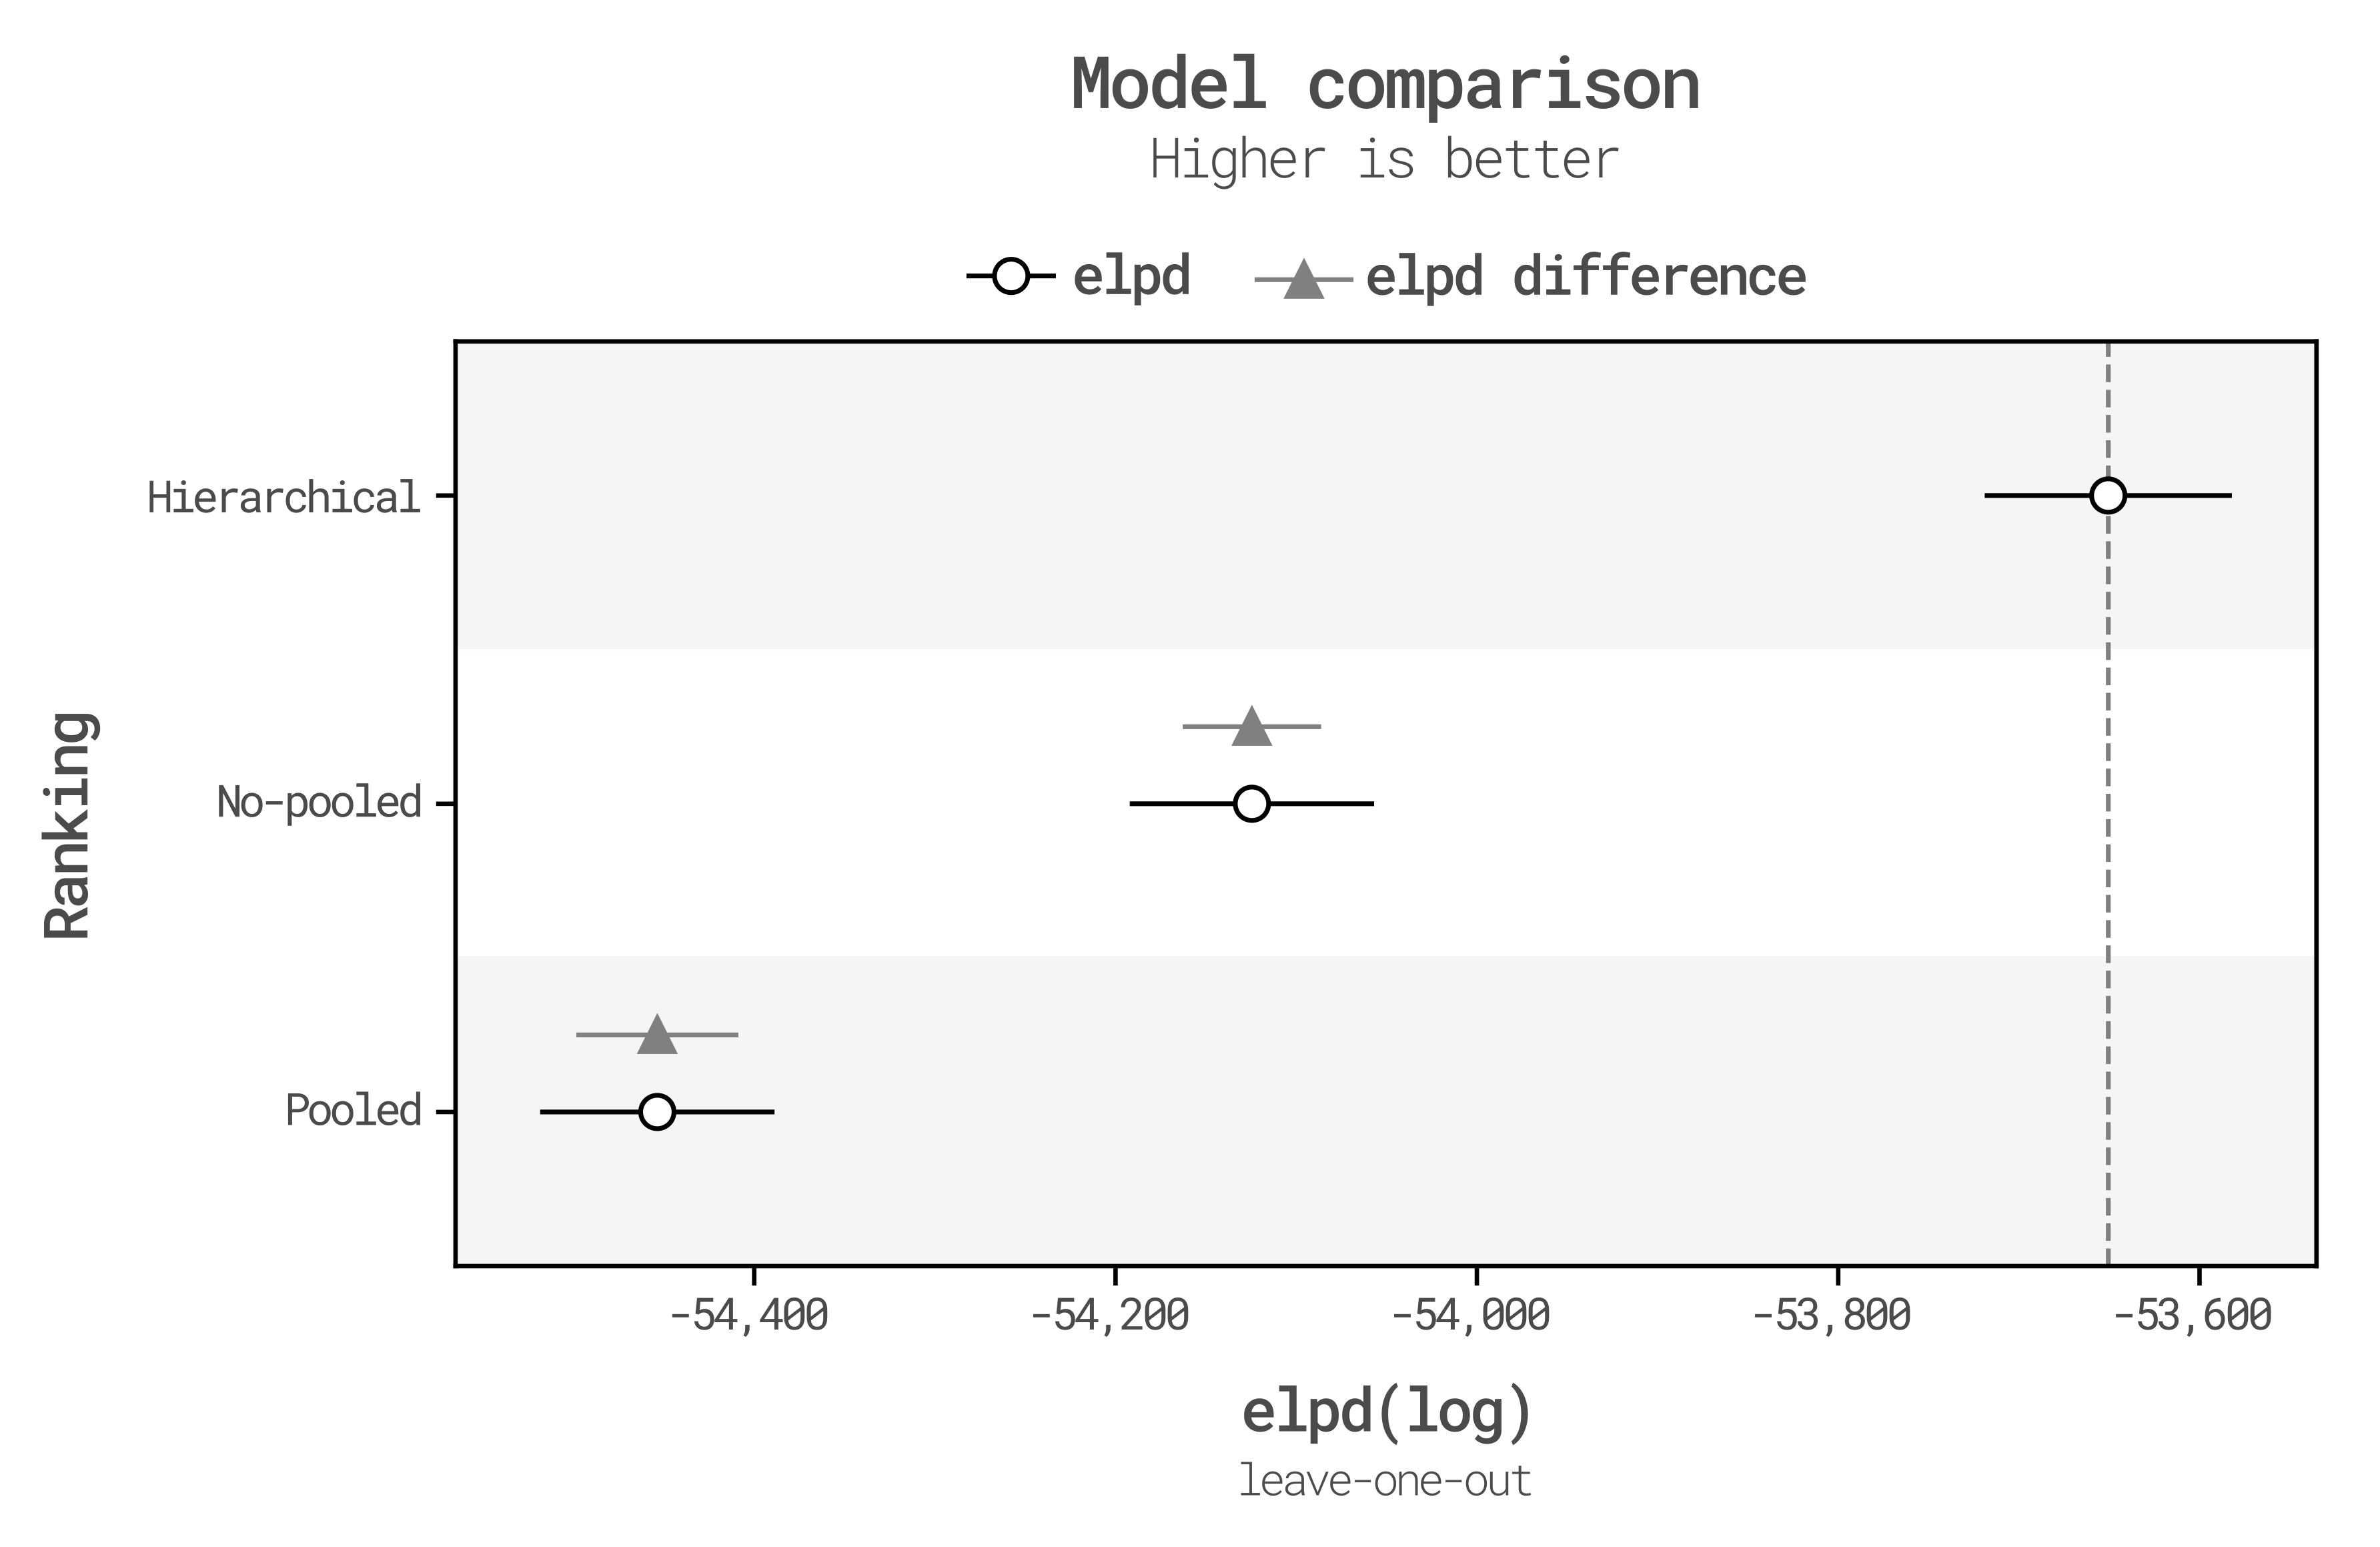
\includegraphics[width=1.0\textwidth]{./images/model_structure_comparison.png}
                \captionsetup{labelformat=empty}
                \setlength{\abovecaptionskip}{-10pt}
                \caption{\fontsize{8pt}{8pt}\selectfont \textbf{\textit{Model performance comparison of proposed structures}}}
            \end{figure}
    \end{columns}
\end{frame}

\begin{frame}{Predicting salaries}{Variable selection}
    \vspace*{-50pt}
    \begin{columns}
        \column{0.4\textwidth}
            \begin{itemize}
                \item \fontsize{10pt}{12pt}\selectfont Experience, Sex, and Education level are the \textbf{most important} predictors.
                \item \fontsize{10pt}{12pt}\selectfont The improvement for adding Age and Self-employment as predictor is \textbf{minimal}.
            \end{itemize}
        \column{0.6\textwidth}
            \begin{figure}
                \centering
                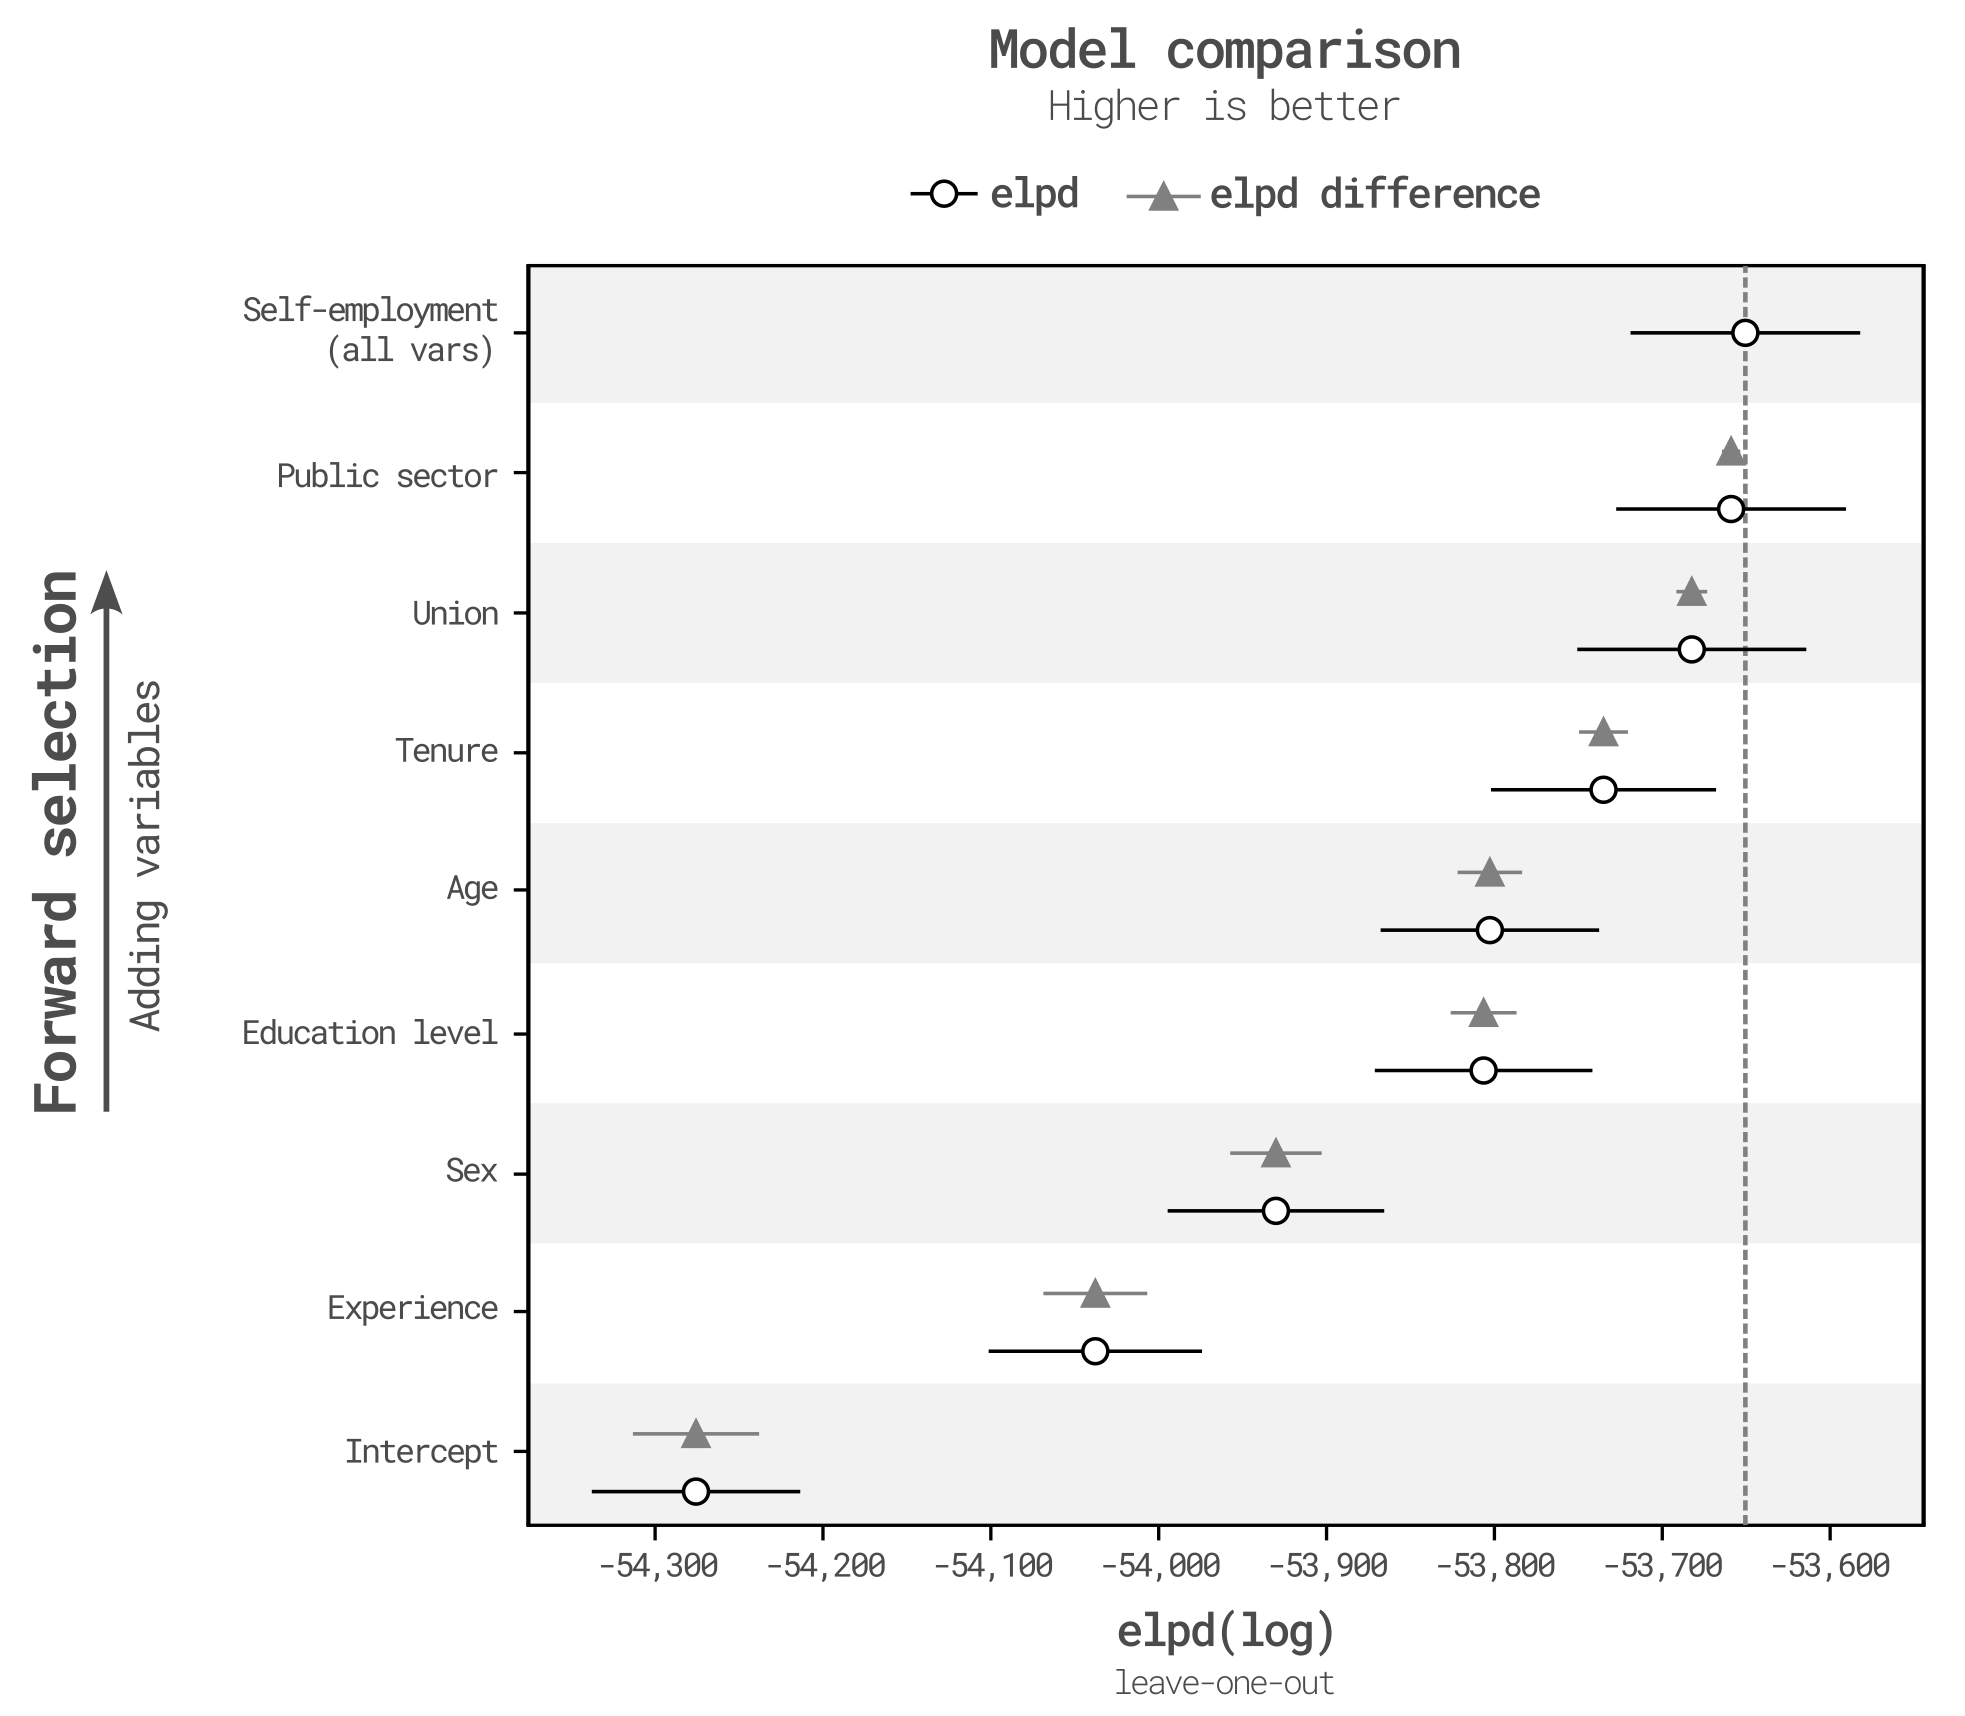
\includegraphics[width=1.0\textwidth]{./images/forward_sel.png}
                \captionsetup{labelformat=empty}
                \setlength{\abovecaptionskip}{-10pt}
                \caption{\fontsize{8pt}{8pt}\selectfont \textbf{\textit{Forward variable selection process}}}
            \end{figure}
    \end{columns}
\end{frame}

{
\setbeamercolor{background canvas}{bg=blue}
\begin{frame}
    \begin{center}
        \textcolor{white}{{\fontsize{22pt}{14pt}\selectfont \textbf{Model validation and results}}}\\
        \vspace{20pt}
        \textcolor{white}{{\fontsize{14pt}{10pt}\selectfont \textsl{Aggregated and disaggregated level}}}
    \end{center}
\end{frame}
}

\begin{frame}{Model validation and results}{Estimated parameters}
    \vspace*{-20pt}
    \begin{columns}
        \column{0.25\textwidth}
        \begin{itemize}
            \item \fontsize{8pt}{12pt}\selectfont The parameters' effect and variability is \textbf{higher} on the occupation level.
            \item \fontsize{8pt}{12pt}\selectfont Experience and education level have a \textbf{positive effect} in salaries.
            \item \fontsize{8pt}{12pt}\selectfont Overall, the \textbf{Gender gap} effect is \textbf{negative}.
        \end{itemize}
        \column{0.75\textwidth}
            \begin{figure}
                \centering
                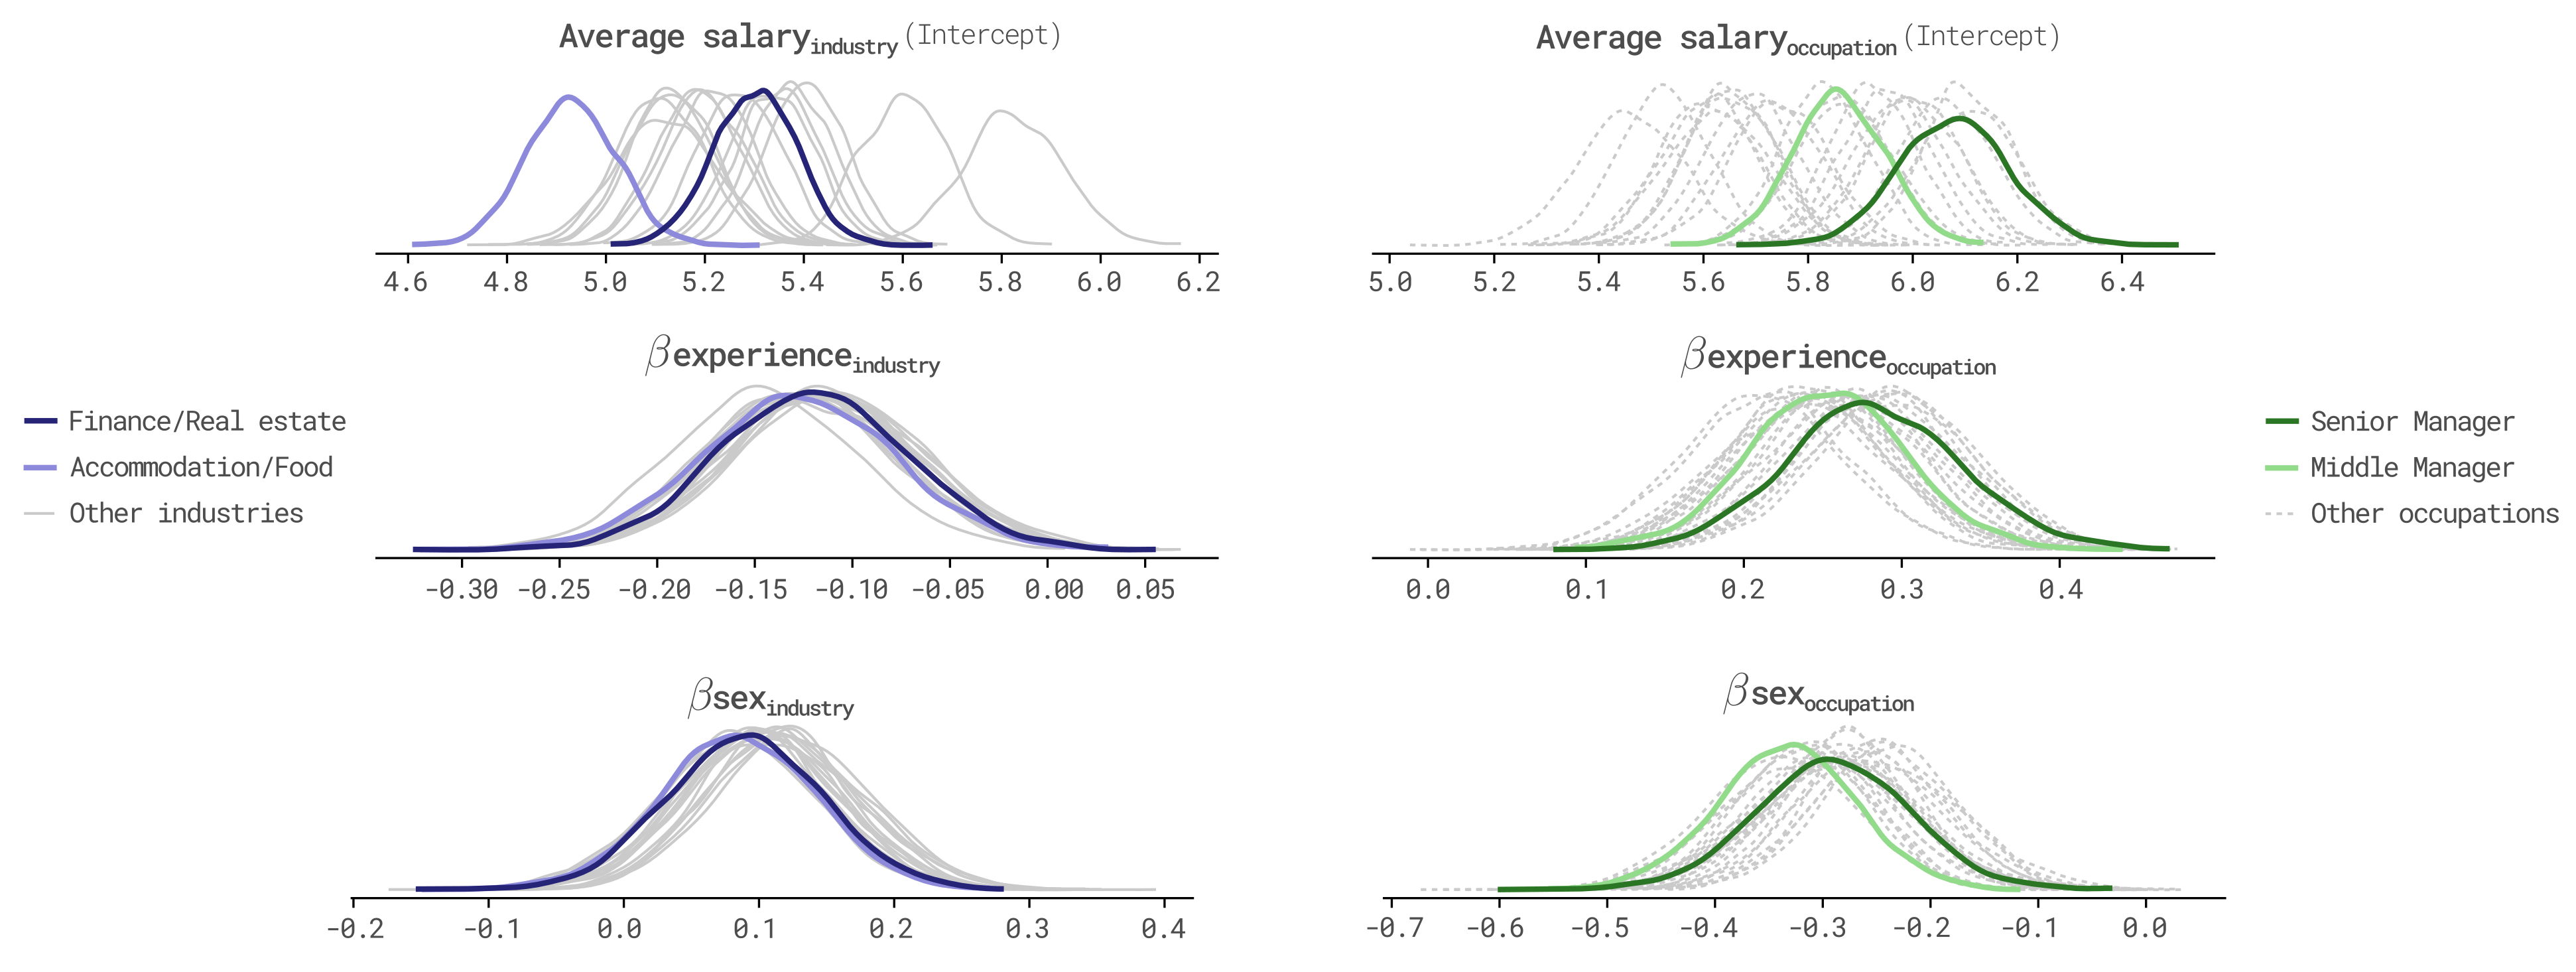
\includegraphics[width=1.05\textwidth]{./images/trace_1.png}
                \captionsetup{labelformat=empty}
                \setlength{\abovecaptionskip}{-10pt}
                \caption{\fontsize{8pt}{8pt}\selectfont \textbf{\textit{Posterior distribution for some model's parameters}}}
            \end{figure}
    \end{columns}
\end{frame}

\begin{frame}{Model validation and results}{Aggregated level - GTA}
    \vspace*{-20pt}
    \begin{columns}
        \column{0.4\textwidth}
            \begin{itemize}
                \item \fontsize{10pt}{12pt}\selectfont The model validation is performed using the \textbf{validation set (2008-2011)}.
                \item \fontsize{10pt}{12pt}\selectfont This data was \textbf{not used} in the model estimation.
                \item \fontsize{10pt}{12pt}\selectfont These results provide a good measure of the \textbf{real model's predictive performance (out-of-sample)}.
            \end{itemize}
        \column{0.6\textwidth}
            \begin{figure}
                \centering
                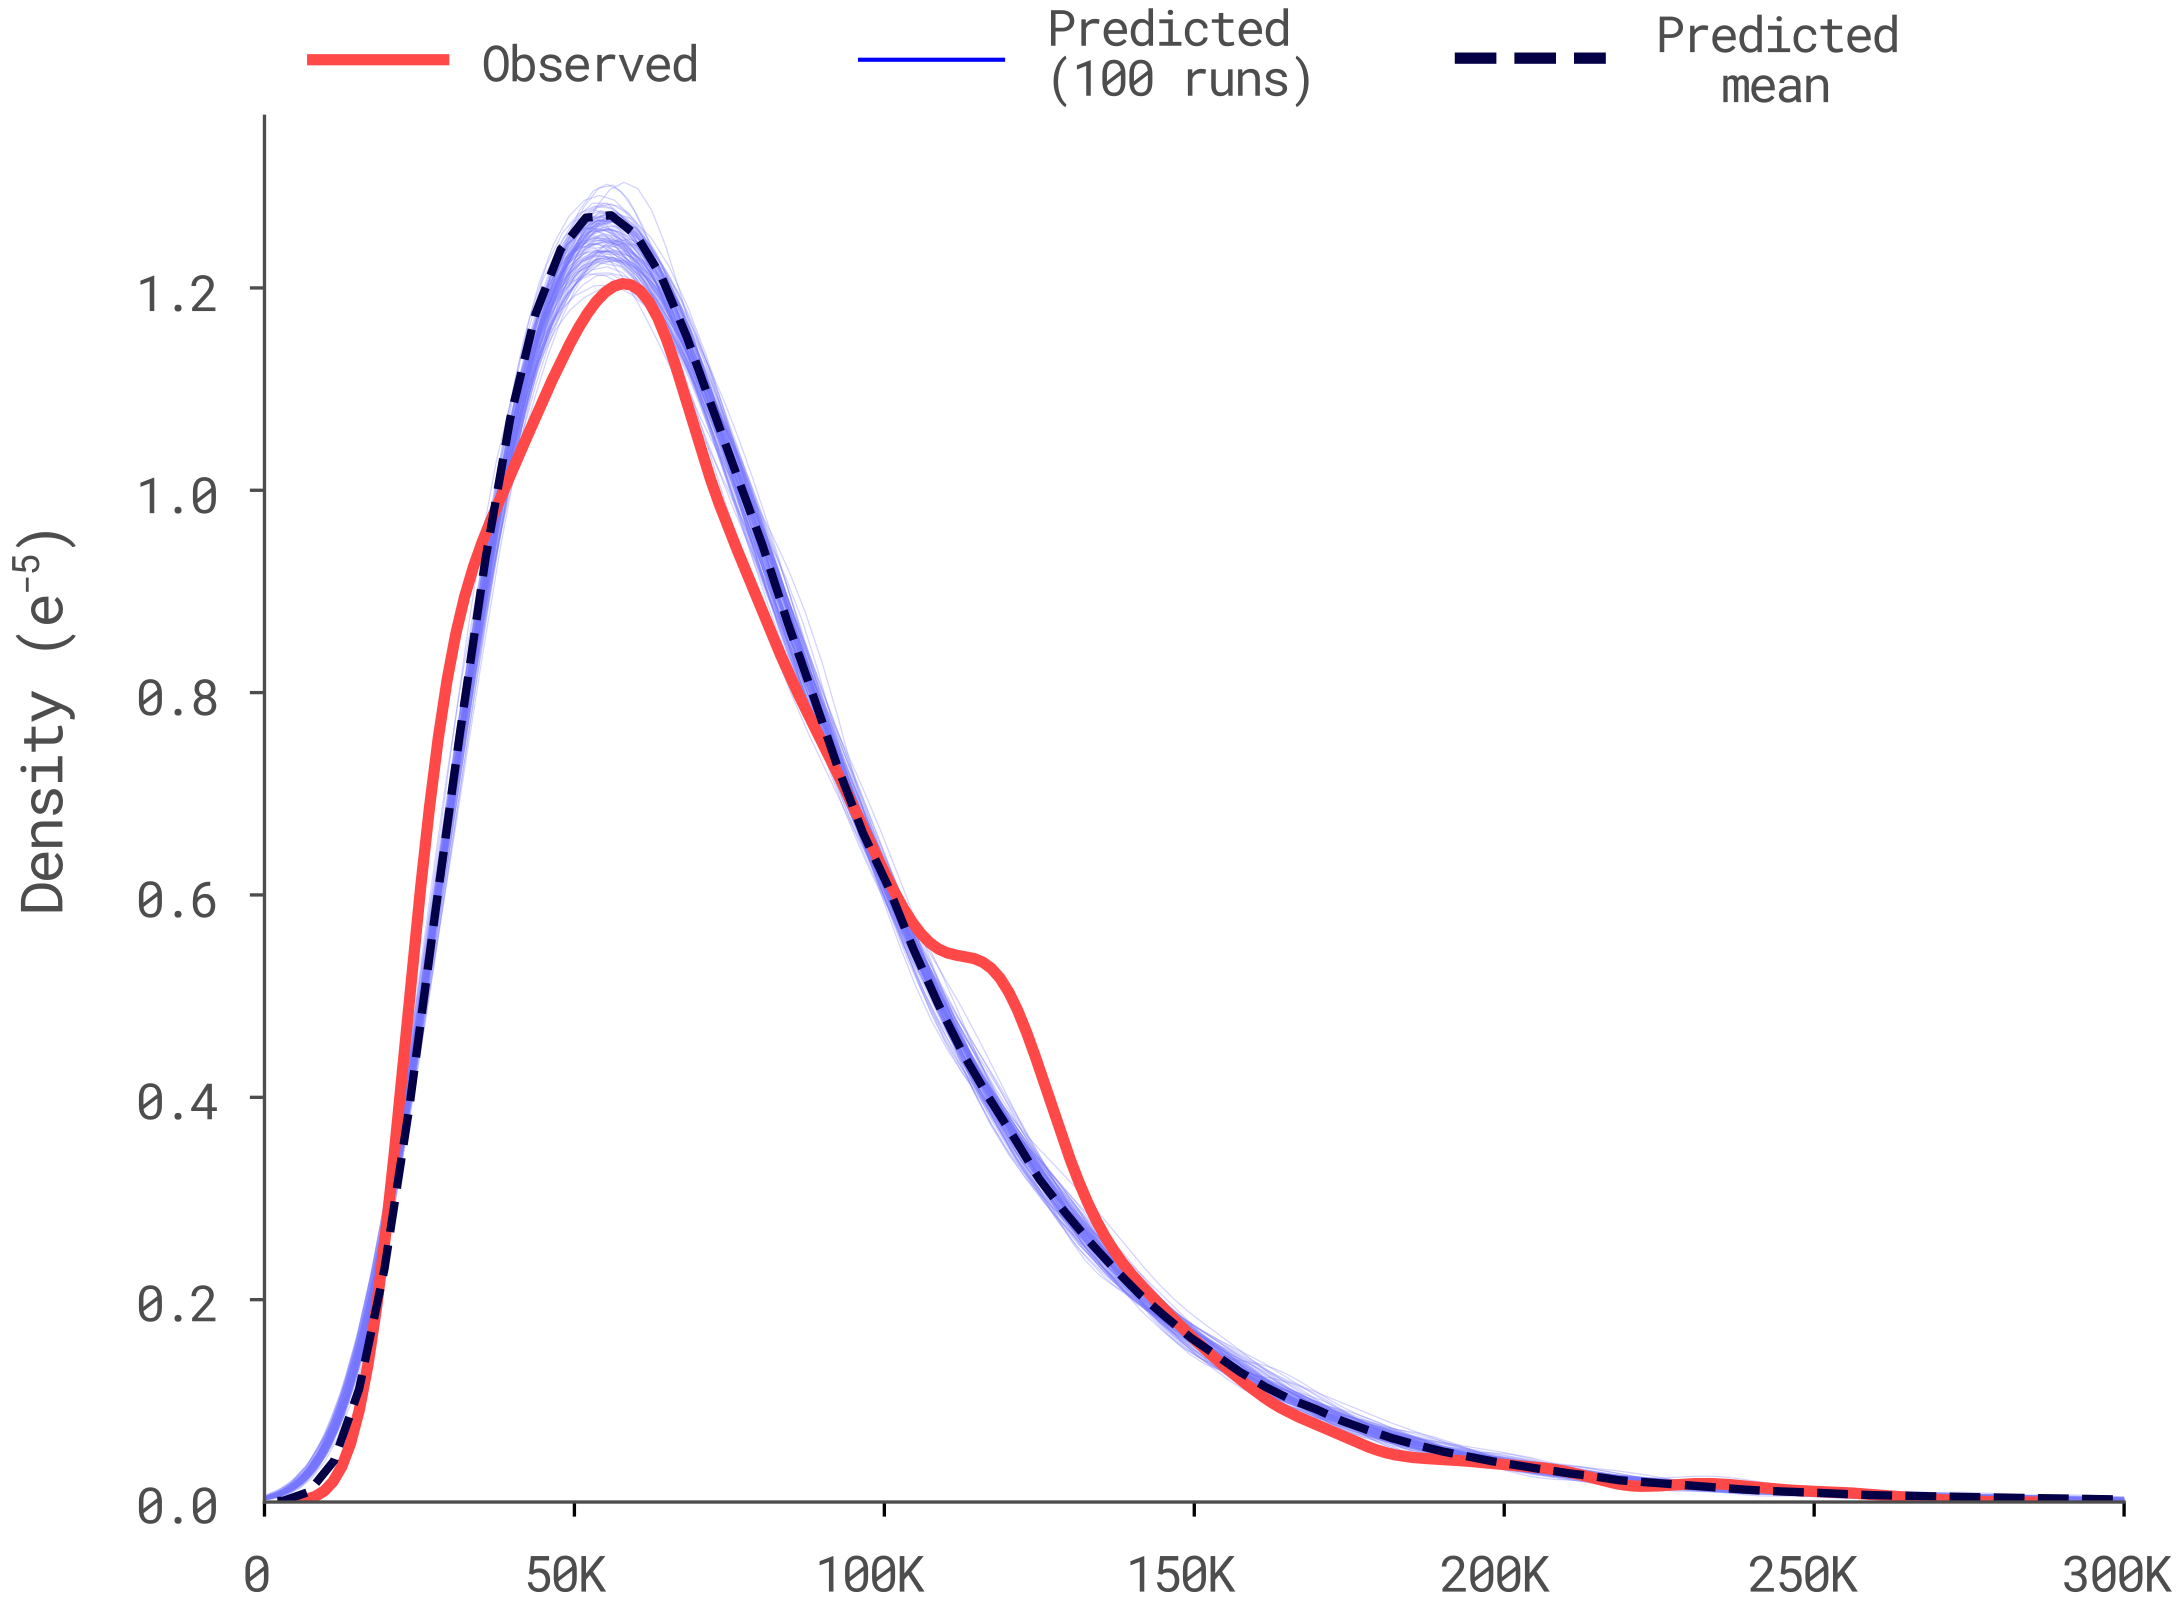
\includegraphics[width=1.0\textwidth]{./images/salary.png}
                \captionsetup{labelformat=empty}
                \setlength{\abovecaptionskip}{-10pt}
                \caption{\fontsize{8pt}{8pt}\selectfont \textbf{\textit{Observed and predicted annual salary distribution for the GTA}}}
            \end{figure}
    \end{columns}
\end{frame}

\begin{frame}{Model validation and results}{Aggregated level - Industry}
    \vspace*{-20pt}
    \begin{figure}
        \centering
        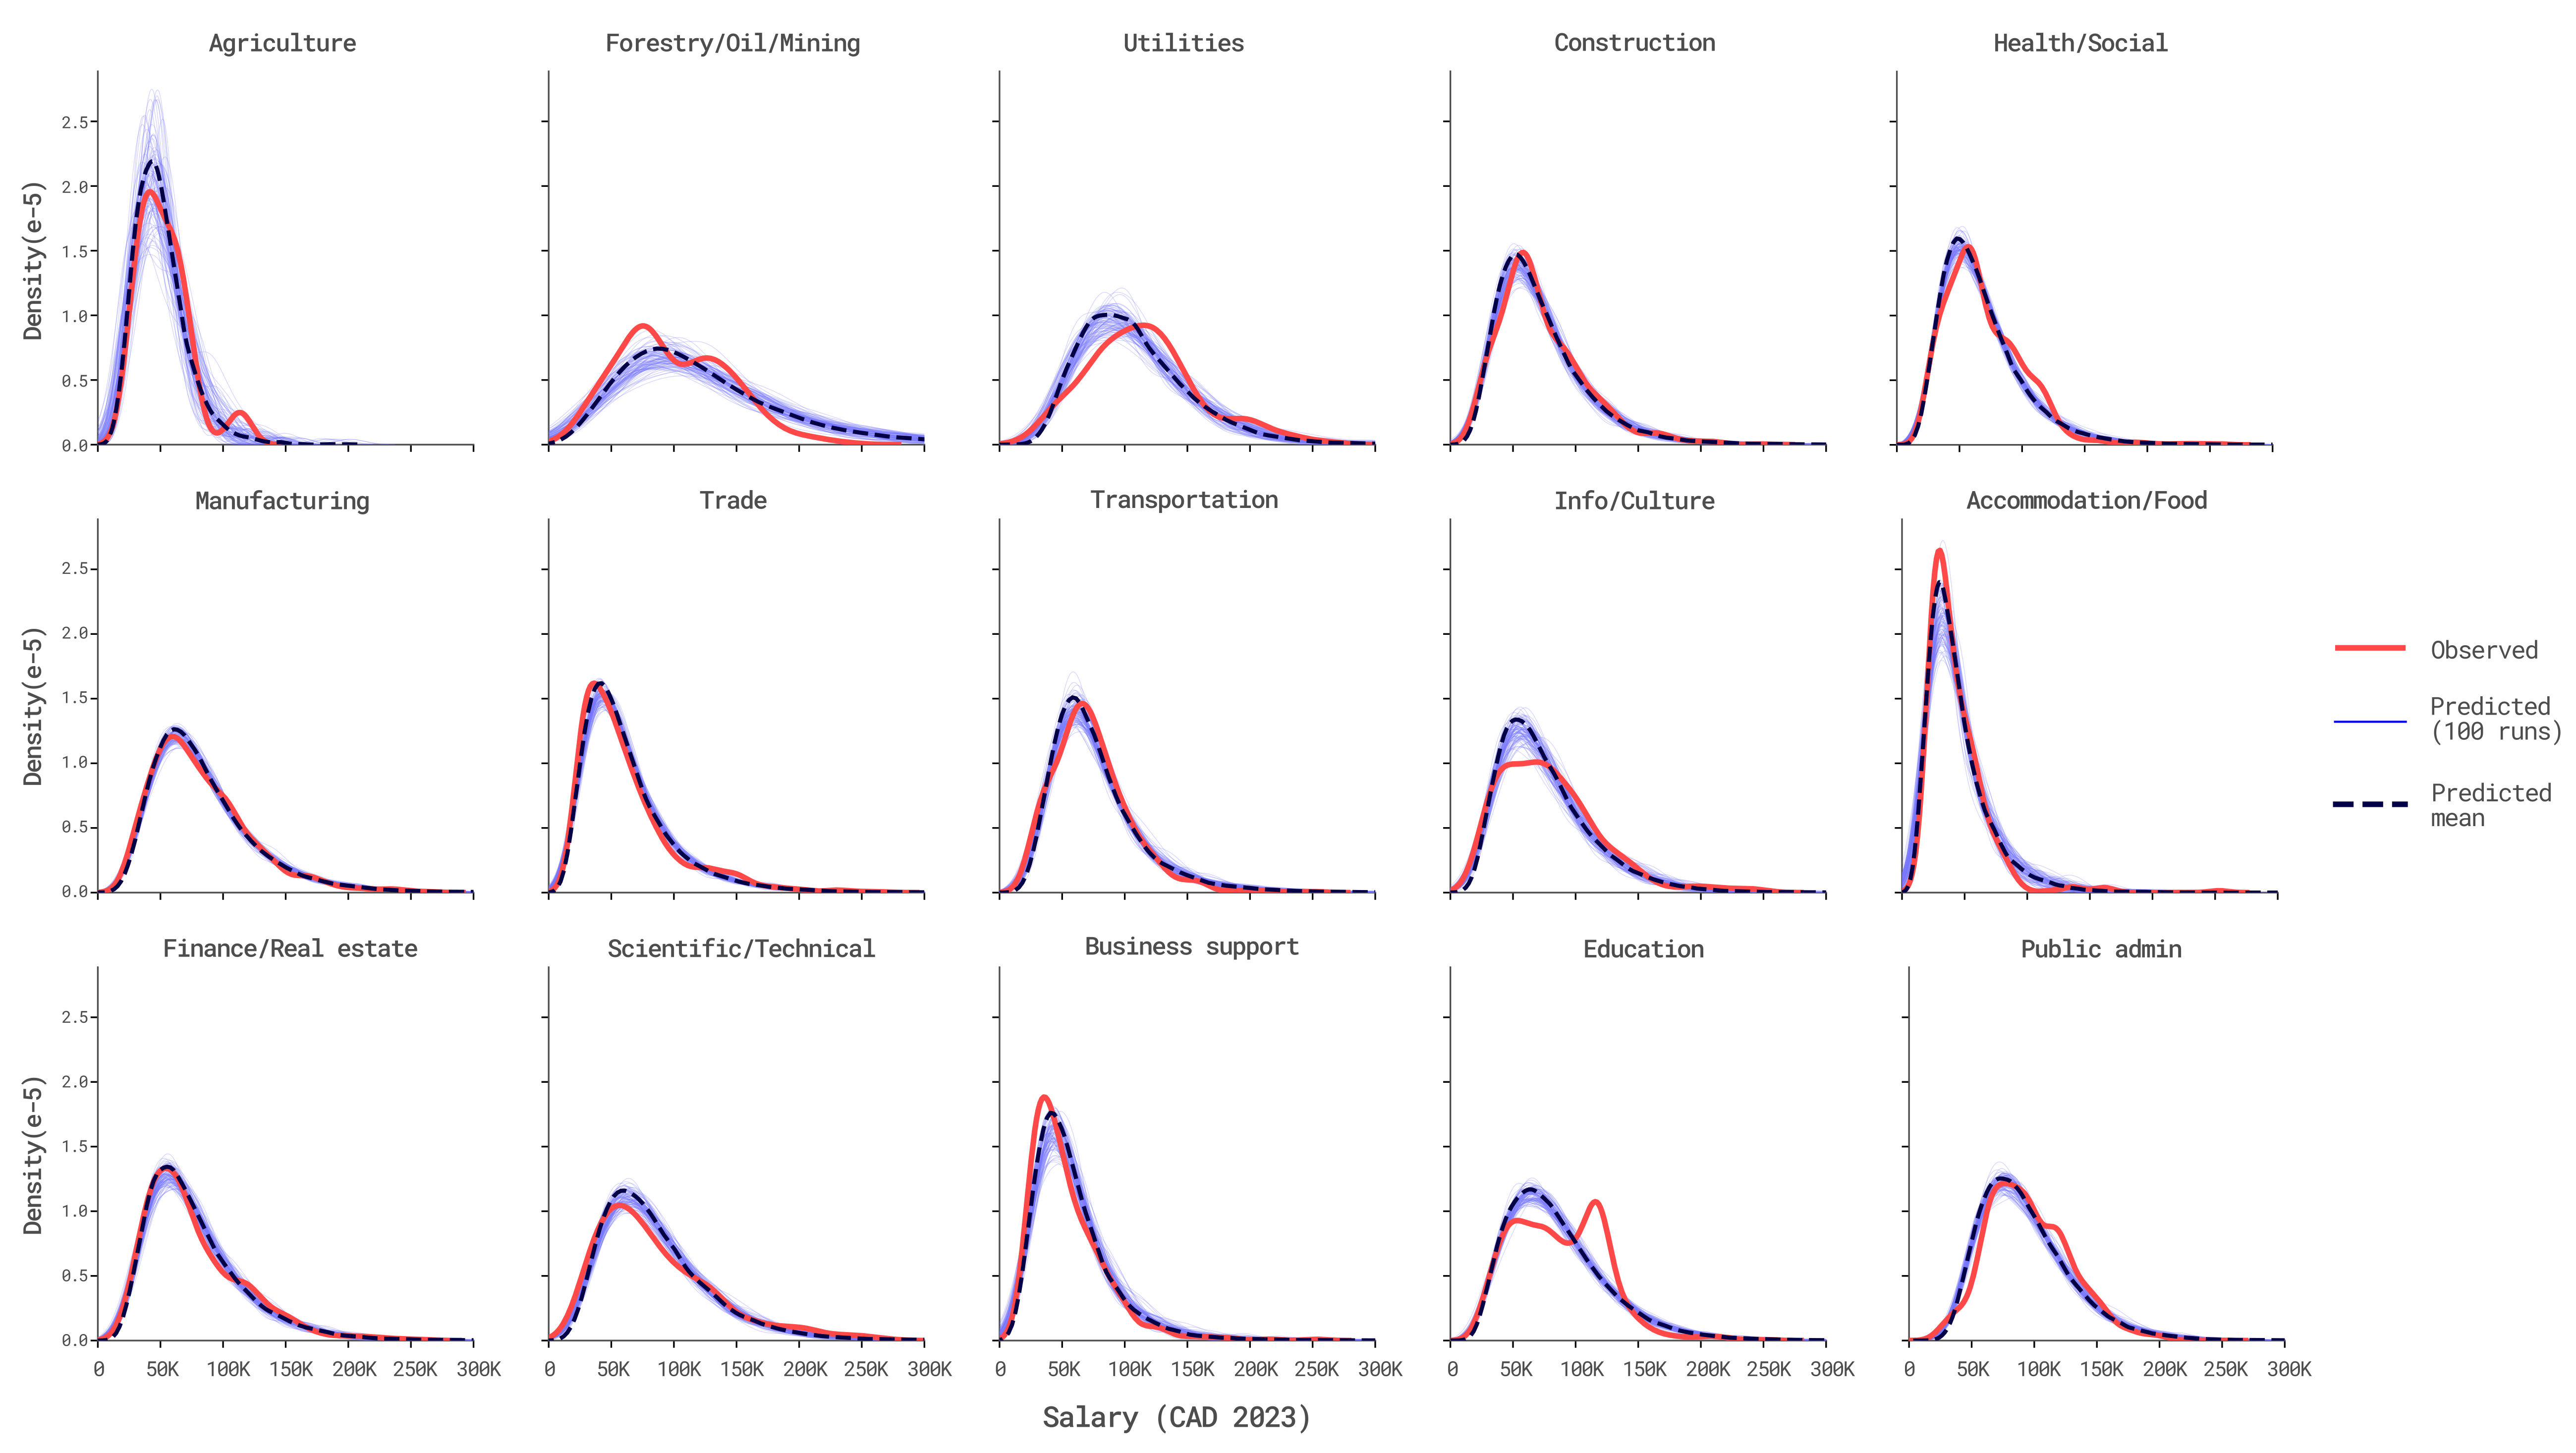
\includegraphics[width=0.8\textwidth]{./images/salary_ind.png}
        \captionsetup{labelformat=empty}
        \setlength{\abovecaptionskip}{-2pt}
        \caption{\fontsize{8pt}{8pt}\selectfont \textbf{\textit{Observed and predicted annual salary distribution by industry for the GTA}}}
    \end{figure}
\end{frame}

\begin{frame}{Model validation and results}{Aggregated level - Occupation}
    \vspace*{-20pt}
    \begin{figure}
        \centering
        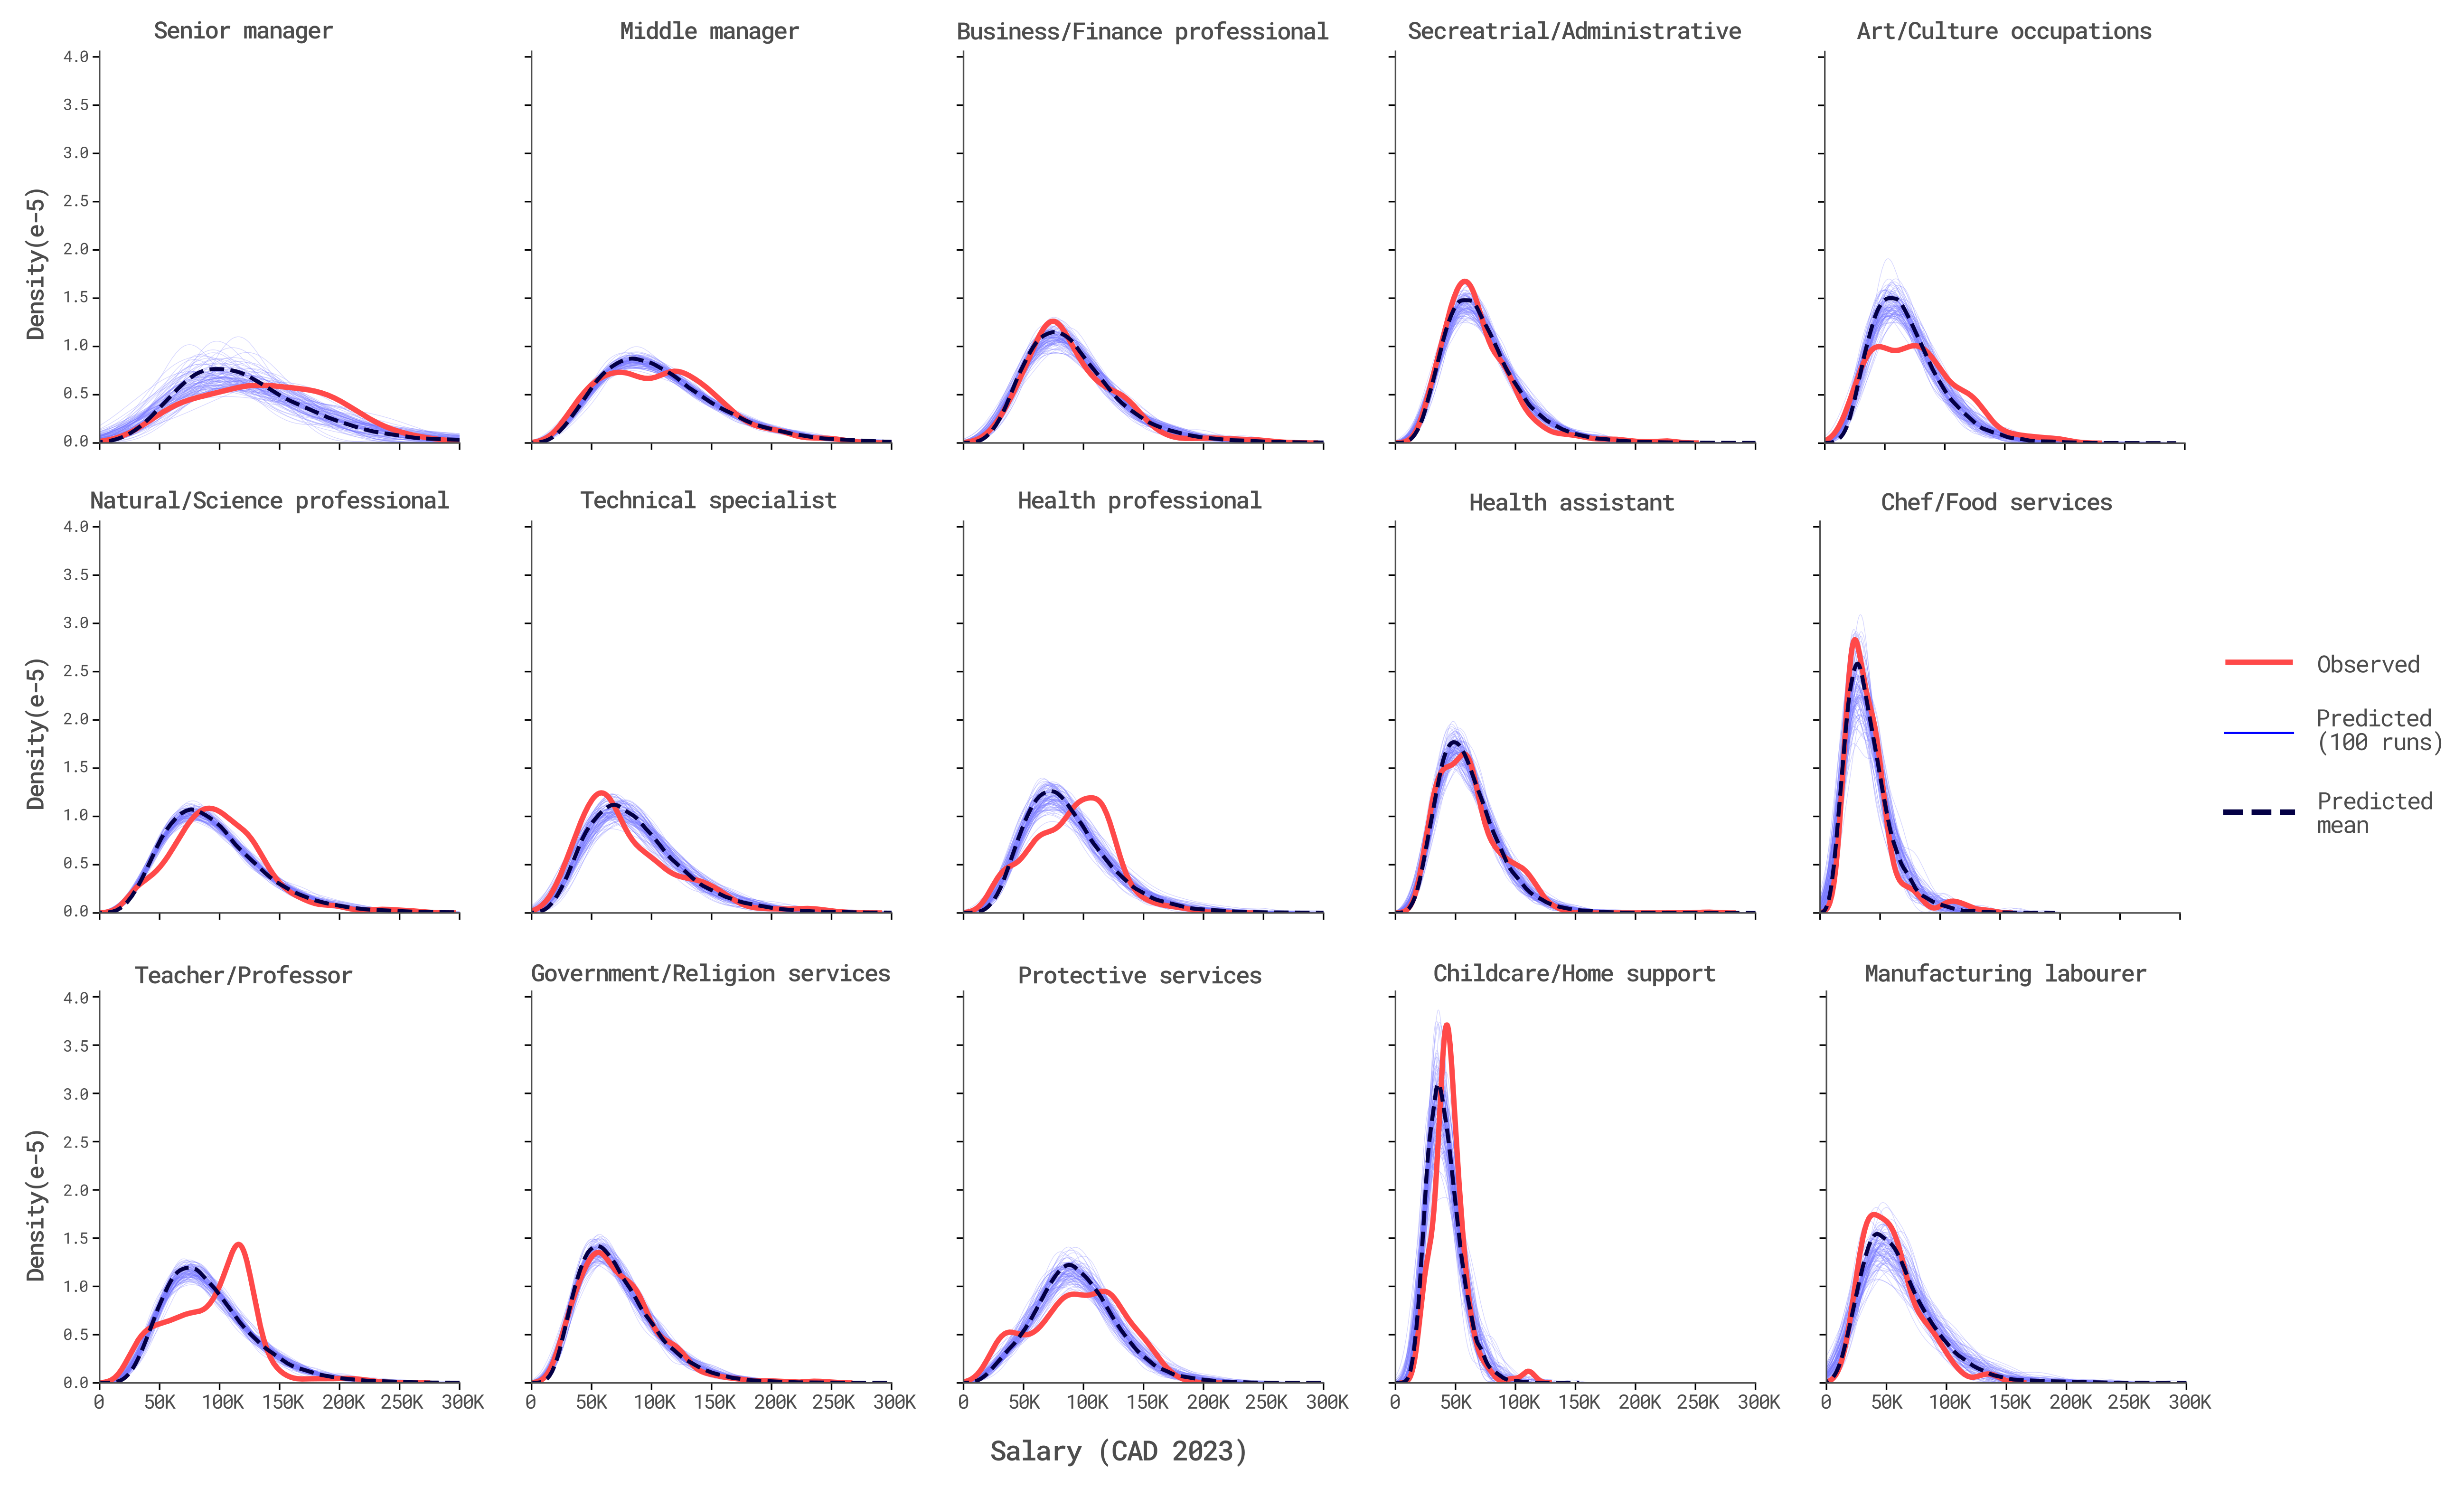
\includegraphics[width=0.8\textwidth]{./images/salary_occ.png}
        \captionsetup{labelformat=empty}
        \setlength{\abovecaptionskip}{-2pt}
        \caption{\fontsize{8pt}{8pt}\selectfont \textbf{\textit{Observed and predicted annual salary distribution by occupation for the GTA}}}
    \end{figure}
\end{frame}

\begin{frame}{Model validation and results}{Disaggregated level}
    \vspace*{-20pt}
    \begin{figure}
        \centering
        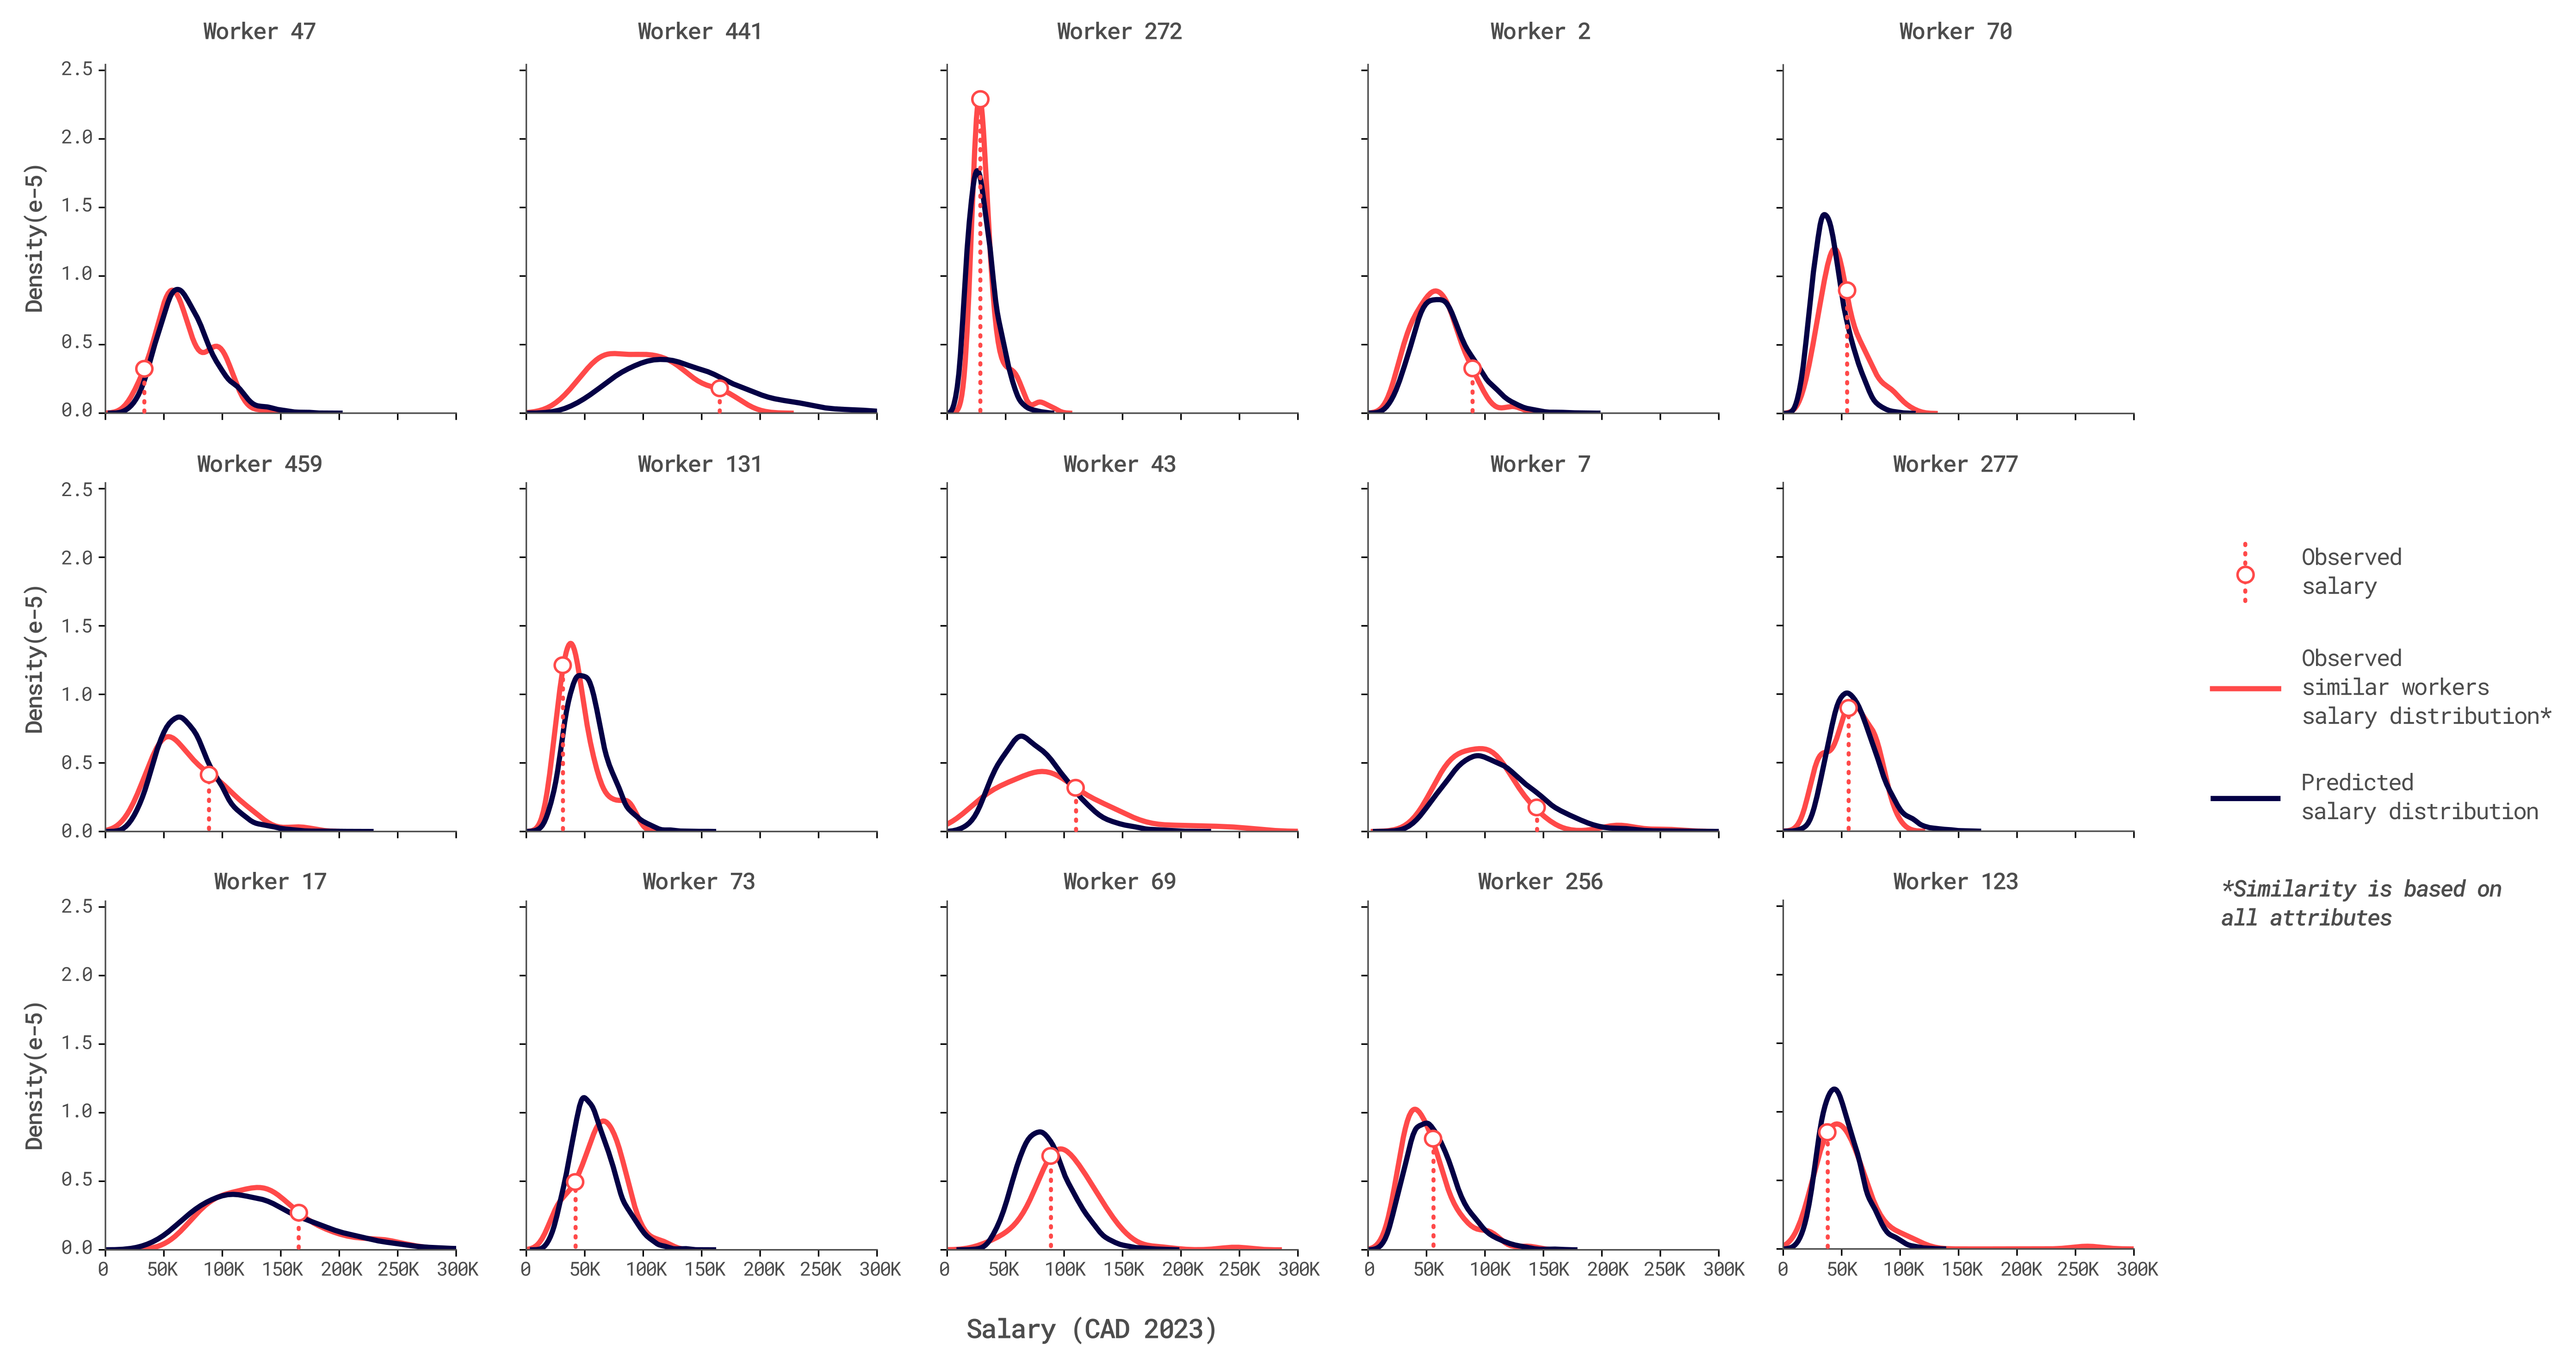
\includegraphics[width=0.9\textwidth]{./images/workers.png}
        \captionsetup{labelformat=empty}
        \setlength{\abovecaptionskip}{-2pt}
        \caption{\fontsize{8pt}{8pt}\selectfont \textbf{\textit{Observed and predicted salaries for a group of randomly selected workers}}}
    \end{figure}
\end{frame}

{
\setbeamercolor{background canvas}{bg=blue}
\begin{frame}
    \begin{center}
        \textcolor{white}{{\fontsize{22pt}{14pt}\selectfont \textbf{Conclusions and future work}}}\\
    \end{center}
\end{frame}
}

\begin{frame}{Conclusions}
    \vspace*{-20pt}
    \begin{itemize}
        \setlength{\itemsep}{10pt}
        \item \fontsize{10pt}{12pt}\selectfont The introduction of the Hierarchical structure in the model allows to capture complex relationships and dependencies in the data. It replaces the manual definition of interaction terms by extracting the information from the data.
        \item \fontsize{10pt}{12pt}\selectfont The definition of the Gamma distribution as the random component of the model allows to capture the data heterogeneity and generate better estimations.
        \item \fontsize{10pt}{12pt}\selectfont Labour markets have some degree of randomness. The use of probability distributions instead of point estimates produces more realistic results.
        \item \fontsize{10pt}{12pt}\selectfont The Bayesian thinking is suitable for modelling complex systems. It allows to update our prior knowledge based on new evidence. However, it comes with a computational cost.
    \end{itemize}
\end{frame}

\begin{frame}{Future work}
    \begin{itemize}
        \item \fontsize{10pt}{12pt}\selectfont Run this model within the Harmon's ABM implementation. \textbf{\textit{Evaluate other submodels to implement the Bayesian approach}}.
        \item \fontsize{10pt}{12pt}\selectfont Include job location as a predictor. \textbf{\textit{Hierarchical models are specially good in spatial applications!}}.
        \item \fontsize{10pt}{12pt}\selectfont Model the parameters' covariance to improve the performance at the disaggregated level. \textbf{\textit{Computationally expensive...For now!}}.
    \end{itemize}
\end{frame}

\begin{frame}{Aknowledgements}
    \fontsize{10pt}{12pt}\selectfont \textit{To my loves: Ale, Emi, Avena. None of this would have been possible without your support}\\
    \vspace{20pt}
    \fontsize{10pt}{12pt}\selectfont \textit{Prof. Eric Miller for his patience, guidance and support during this journey. Cities as complex systems course changed the way I see the world.}\\
    \vspace{20pt}
    \fontsize{10pt}{12pt}\selectfont \textit{COLFUTURO for providing the partial funding for my studies.}\\
    \vspace{20pt}
    \fontsize{10pt}{12pt}\selectfont \textit{Prof. Matthew Roorda for kindly accepting to read this thesis.}\\
    \vspace{20pt}
    \fontsize{10pt}{12pt}\selectfont \textit{TMG group: I learned a lot from you guys. Thanks for the support and the good times!}
\end{frame}

{
\setbeamercolor{background canvas}{bg=blue}
\begin{frame}
    \begin{center}
        \textcolor{white}{{\fontsize{22pt}{14pt}\selectfont \textbf{Questions?}}}\\
        \vspace{20pt}
        \textcolor{white}{{\fontsize{14pt}{10pt}\selectfont \textsl{Thank you for your attention!}}}
    \end{center}
\end{frame}
}
\end{document}